%% 
%% Copyright 2019-2021 Elsevier Ltd
%% 
%% This file is part of the 'CAS Bundle'.
%% --------------------------------------
%% 
%% It may be distributed under the conditions of the LaTeX Project Public
%% License, either version 1.2 of this license or (at your option) any
%% later version.  The latest version of this license is in
%%    http://www.latex-project.org/lppl.txt
%% and version 1.2 or later is part of all distributions of LaTeX
%% version 1999/12/01 or later.
%% 
%% The list of all files belonging to the 'CAS Bundle' is
%% given in the file `manifest.txt'.
%% 
%% Template article for cas-sc documentclass for 
%% single column output.

% Document Class
\documentclass[a4paper,fleqn]{cas-sc}

% Packages
%%\usepackage[authoryear,longnamesfirst]{natbib}
\usepackage[numbers]{natbib}
\usepackage[nodots,nocompress]{numcompress}

%Package to hold figure in position
\usepackage{placeins}

%Author macros
\def\tsc#1{\csdef{#1}{\textsc{\lowercase{#1}}\xspace}}
\tsc{WGM}
\tsc{QE}

\begin{document}
\let\WriteBookmarks\relax
\def\floatpagepagefraction{1}
\def\textpagefraction{.001}

% Short title
\shorttitle{Numerical analysis of the rock deformation in twin tunnels with transverse gallery}    

% Short author
\shortauthors{Quevedo et al.}  

% Main title of the paper
\title [mode = title]{Numerical analysis of the rock deformation in twin tunnels with transverse gallery considering plasticity and time-dependent constitutive models}  

% First author
\author[1]{Quevedo, F. P. M.}[style = chinese, orcid = 0000-0003-4171-1696]
\cormark[1] 					
\cortext[cor1]{Corresponding author.}
\ead{motta.quevedo@ufrgs.br}
\ead[url]{https://www.researchgate.net/profile/Felipe-Pinto-Da-Motta-Quevedo}

% Second author
\author[1]{Colombo, C. A. M. M.}[style=chinese]
\ead{ca-colombo@hotmail.com}
\ead[url]{http://lattes.cnpq.br/4919388217690564}

% Third author
\author[1]{Bernaud, D.}[style=chinese, orcid=0000-0001-6365-3269]
\ead{denise.bernaud@ufrgs.br}
\ead[url]{http://lattes.cnpq.br/2809615143819128}

% Four author
\author[1]{Maghous, S.}[style=chinese, orcid=0000-0002-1123-3411]
\ead{samir.maghous@ufrgs.br}
\ead[url]{https://www.researchgate.net/profile/Samir-Maghous}

% Afilliation
\affiliation[1]{organization={Federal University of Rio Grande do Sul},
	addressline={Av. Osvaldo Aranha, 99}, 
	city={Porto Alegre},
	postcode={90.035-190}, 
	state={RS},
	country={Brazil}}

% Mathematical Symbols
\newcommand{\dgds}{\boldsymbol{g_\sigma}}
\newcommand{\Dll}{\boldsymbol{D}}
\newcommand{\Dllmod}{\boldsymbol{D^{*}}}
\newcommand{\Dllepvp}{\boldsymbol{D}^{epvp}}
\newcommand{\dstrain}{\boldsymbol{\dot{\varepsilon}}}
\newcommand{\dstraine}{\boldsymbol{\dot{\varepsilon}}^{e}}
\newcommand{\dstrainp}{\boldsymbol{\dot{\varepsilon}}^{p}}
\newcommand{\dstrainv}{\boldsymbol{\dot{\varepsilon}}^{vp}}
\newcommand{\straineqp}{\bar \varepsilon^p}
\newcommand{\dstrainsh}{\boldsymbol{\dot{\varepsilon}}^{sh}}
\newcommand{\dstraincr}{\boldsymbol{\dot{\varepsilon}}^{cr}}
\newcommand{\dstress}{\boldsymbol{\dot{\sigma}}}

\newcommand{\ex}{\boldsymbol{e}_x}
\newcommand{\ey}{\boldsymbol{e}_y}
\newcommand{\ez}{\boldsymbol{e}_z}

\newcommand{\onell}{\boldsymbol{1}}
\newcommand{\strain}{\boldsymbol{\varepsilon}}
\newcommand{\straincr}{\boldsymbol{\varepsilon}^{cr}}
\newcommand{\straine}{\boldsymbol{\varepsilon}^{e}}
\newcommand{\strainp}{\boldsymbol{\varepsilon}^{p}}
\newcommand{\strainsh}{\boldsymbol{\varepsilon}^{sh}}
\newcommand{\strainshCEB}{\varepsilon_{sh}}
\newcommand{\strainvp}{\boldsymbol{\varepsilon}^{vp}}
\newcommand{\stress}{\boldsymbol{\sigma}}
\newcommand{\zerol}{\boldsymbol 0}

% Here goes the abstract
\begin{abstract}
Resorting to a three-dimensional finite element framework, the paper investigates the instantaneous and long-term deformation in twin tunnels with connecting transverse gallery. Particular emphasis is dedicated to assessment of combined effects induced by time-dependent constitutive behavior of the material constituents and twin tunnels proximity, on the convergence profile. At the material level, the rock material mechanical behavior is formulated within the context of coupled plasticity–viscoplasticity, which proves relevant to the modeling and simulation of tunnel deformation in deep clayey rocks.  A fundamental aspect of modeling the rock/support structure mechanical interaction is related to the proper consideration of time-dependent properties of the lining concrete material.  In that respect, the concrete creep deformation is addressed by means of an aging viscoelastic model relying on the Bažant and Prasannan Solidification Theory, whereas shrinkage deformation component is accounted for by means of the formulation proposed in CEB-FIP MC90 standard. At the structure level, the deactivation-activation technique is employed in the three-dimensional computational model to simulate the excavation/advancing face and lining installation processes. The accuracy of the finite element predictions is assessed through comparisons with available analytical stress solutions formulated within a simplified setting for the twin tunnels configuration. The computational model is applied to analyze the short-term and long-term convergence profiles in a fully 3D twin tunnels configuration.  A series of simulations varying some relevant parameters defining the structure geometry and constituents behavior are undertaken with the aim to give preliminary insight into the multiple interactions rising from twin tunnel proximity, intersecting transverse gallery and lining support. Numerical simulations have notably emphasized the deformation anisotropy induced by tunnels proximity as well as that peak convergence values are observed within a localized extension region close to tunnel-gallery intersection. Finally, the crucial role of time-dependent properties of concrete lining and related instantaneous stiffness in controlling the tunnel deformation is also studied.
\end{abstract}

% Use if graphical abstract is present
\begin{graphicalabstract}
	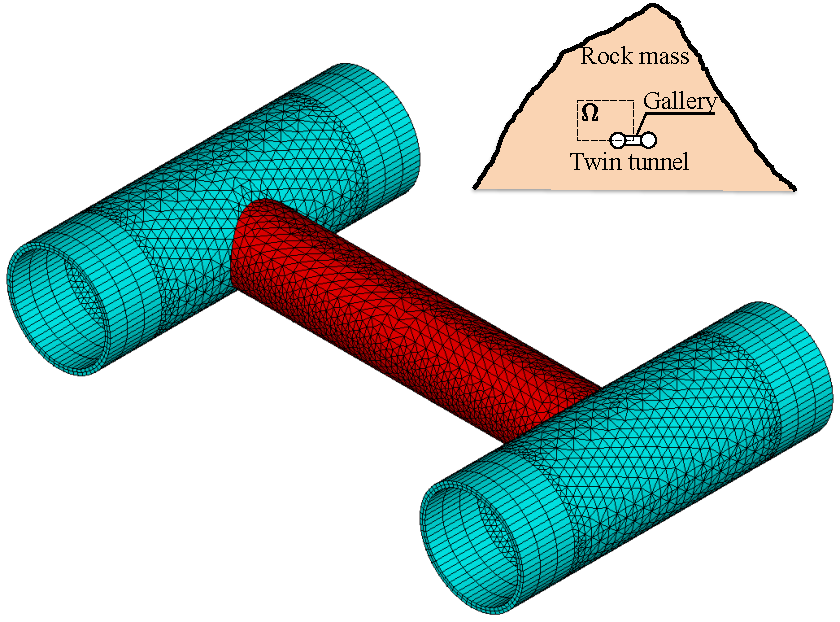
\includegraphics[scale=1]{graphical_abstract.pdf}
\end{graphicalabstract}

% Research highlights
\begin{highlights}
	\item Rock deformation in twin tunnels with transverse gallery is addressed by 3D computational.
	\item The irreversible behavior of the rock material is formulated in the context of coupled plasticity-viscoplasticity.
	\item Creep deformation o lining concrete is addressed by aging viscoelastic model.
	\item Numerical simulations emphasize the tunnel deformation anisotropy induced by twin tunnels proximity.
	\item High lining instantaneous stiffness can predominately control tunnel convergence and restrict interaction effects.
\end{highlights}

% Keywords
\begin{keywords}
twin tunnels \sep transverse gallery \sep plasticity-viscoplasticity coupling
\sep viscoelastic lining \sep finite element model
\end{keywords}

\maketitle

\section{Introduction}\label{}

The increasing development of tunnel infrastructures for transportation systems and facilities networks in urban, hilly or underwater environments requires rational and efficient use of underground space, leading in many situations to tunneling nearby existing or new tunnels. The number of deep or shallow twin tunnels excavated in close proximity to each other has notably increased in the last years mainly due to prevailing underground and geotechnical conditions in congested urban areas. Resorting to the solution of twin tunnels, each branch being devised for a flow direction, also presents technical and safety advantages such as the reduction of tunnel diameter. Furthermore, in most cases of adjacent twin tunnels, the construction of connecting transverse galleries is a standard tunnel engineering practice either for safety (emergency exit/access) or functionality (maintenance, service cross-passage) purposes.

The sequence of construction phases of parallel twin tunnels running side-by-side as well as of the transverse gallery is generally dictated by the engineering practice and construction program. The tunnel junctions are usually constructed far behind the advancing face of main tunnel to ensure the excavation of latter slightly affects that of the junction gallery [\citenum{chortis2021b},\citenum{insam2019}]

In this context, understanding and assessing the multiple interactions between the components of such a tunnel material system, namely the closely-spaced twin tunnels, the intersecting transverse gallery, the support lining and the ground, is a fundamental and challenging engineering issue that should be handled during the planning stages for optimal design and safety of the whole tunneling operations. Evidence of interaction phenomena in twin tunnels and tunnel junctions have been reported by many case studies (e.g., \citenum{pottler1992}, \citenum{nyren1998}, \citenum{hsiao2005}, \citenum{sjoberg2006}, \citenum{karakus2007}, \citenum{afifipour2011}, \citenum{Fortsakis2012}, \citenum{fargnoli2015}, \citenum{li2016}, \citenum{elwood2016}, \citenum{connor2016}, \citenum{wan2017}, \citenum{insam2019}]. From a structural design viewpoint, the analysis of the complex interaction in such a tunnel system is not an easy task since it inherently involves several factors related to geometry and constitutive characteristics as well as to the prevailing initial mechanical state and the sequence of tunneling. In particular, the computational evaluation of rock deformation and lining loading near the region of tunnel-gallery intersection requires a three-dimensional modeling (e.g., [\citenum{spyridis2015}, \citenum{chortis2021a}]. The construction process of the transverse gallery induces a stress redistribution within the surrounding rock mass, which in turn results in additional loading applied to the lining support of the main tunnel. Furthermore, a key aspect of the 3D modeling is the ability to capture the interaction effects on both short-term and long-term structural behavior, which are mainly controlled by the time-dependent rheological behavior of the rock and lining material constituents.

As far as the computational tunnel interaction modeling is concerned, most investigations addressed the configuration of shallow adjacent or twin tunnels (see for instance [\citenum{karakus2007}, \citenum{ZHENG2015}, \citenum{do_three-dimensional_2014}, \citenum{do_3d_2016}, \citenum{vlachopoulos2018}, \citenum{forsat2022}, \citenum{do_numerical_2022},  \citenum{pedro2022}, \citenum{PHUTTHANANON2023}], to cite a few recent works), with particular focus on subsurface and surface interaction effects, including evaluation of induced ground settlement. In that respect, a comprehensive review of reference works on related topics may be found in [\citenum{ISLAM2021}].

Referring to the particular configuration of deep-buried tunnels addressed in this paper, the following analytical and numerical contributions to twin tunnels interaction modeling should be quoted. Analytical solutions for the stress distribution around unlined and lined deep circular twin tunnels have been respectively formulated in [\citenum{GUO2021}] and [\citenum{Chen2019}] within the framework of plane strain assumption considering an elastic behavior for the rock material. It has been found that the interaction between the twin tunnels vanishes when the tunnel spacing exceeds typically two to three tunnel diameters. Similar problem has been studied in [\citenum{MA2020}] who considered unlined deep twin circular tunnels excavated in a homogeneous elastoplastic medium. The approximate analytical solution formulated for the stresses and the plastic zone extent has been verified through comparison with numerical results using FLAC3D software. The authors carried out a parametric study to assess the influence of twin tunnels spacing, rock strength properties and in-situ initial stresses on the shape and extent of the plastic zones.

Several 3D numerical analyses have investigated the mechanical interaction in deep adjacent tunnels (see for instance [\citenum{chen2009}, \citenum{Fortsakis2012}, \citenum{vlachopoulos2014}, \citenum{shaofeng2018}, \citenum{chortis2021b}], among others). One may refer to [\citenum{chortis2021b}] for a more exhaustive review on 3D computational approaches dealing with such a problem. Overall, most of these studies emphasized the crucial effect of pillar width on interaction phenomena occurring in the area between adjacent tunnels. The numerical simulations also indicated that the redistribution of strains and stresses induced in the zone between adjacent tunnels by the construction process may be fundamental to devise adequate support/lining system [\citenum{Fortsakis2012}, \citenum{chortis2021b}]. In this context, Chortis and Kavvadas [\citenum{chortis2021b}] carried out parametric 3D finite element analyses to assess the interaction between deep parallel twin tunnels, with circular and non-circular cross-section, excavated in an elastoplastic rock mass and supported by a linear elastic shotcrete lining. The study focused the interaction analysis on the axial forces that develop in the primary lining of the twin tunnels by considering the effects of geometrical, geotechnical and material constitutive parameters as well as of the construction conditions . In addition, an important conclusion drawn from these studies is that 2D analyses cannot realistically capture the purely 3D interaction nature of the tunneling problem [\citenum{vlachopoulos2014}].

However, few numerical works addressed the interaction phenomena associated with the excavation of transverse gallery connecting the main tunnels. This is mainly due to the fact the numerical simulation of the tunnel junction area would rely on complex 3D geometry discretization together with a large number of calculation steps to provide realistic modeling of the sequentially tunneling process, thus leading to time-consuming procedures. Recent representative works include references [\citenum{hsiao2009}, \citenum{spyridis2015}, \citenum{li2016}, \citenum{liu2017}, \citenum{chortis2021a}, \citenum{chortis2023b}, \citenum{chortis2023b}]. As reported in [\citenum{chortis2021a}], the interaction between the transverse gallery and the main longitudinal tunnels significantly modifies the deformation and stress states of the primary support and the surrounding rock mass at the intersection area, making 3D numerical simulations necessary for the realistic design of such complex structure. It is pointed out that most of the numerical studies were limited to case studies and, as such, cannot be provide design guidelines for more general tunnel junctions. In that respect, on should particularly quote the contributions by Chortis and Kavvadas [\citenum{chortis2021a}, \citenum{chortis2023b}, \citenum{chortis2023a}] who investigated the mechanical interaction in deep tunnel junction by means of 3D finite element analyses. Based on a comprehensive set of parametric 3D finite element studies, these authors formulated design charts for the axial forces and bending moments acting on the primary support in the intersection zone between the main and junction tunnels.

Existing literature addressing the mechanical interaction in deep twin tunnels with connecting transverse galleries has mainly focus on the response associated with instantaneous reversible/irreversible behavior of the rock mass and lining constituent materials. It is however well established that creep is an essential component of rock deformation in deep tunnels, leading to progressive development of tunnel convergence and lining loading during the construction phase and extending over months or even years.  In this context, the purpose of the present study is to investigate the implications of time -dependent constitutive properties of rock and support shotcrete/concrete materials on the short-term and long-term structural behavior.  At the material level, the 3D computational model integrates the constitutive state equations formulated for the rock in the framework of coupled plasticity-viscoplasticity, which proves relevant for capturing both irreversible instantaneous response (plasticity) as well as the delayed irreversible response (viscoplasticity). Creep behavior of the lining material, typically shotcrete, is described by means of an aging viscoelastic model that notably accounts for the properties at early age. At the tunnel structure level, the constitutive modeling and related as well as the related numerical integration schemes are developed and implemented within a specific UPF/USERMAT procedure of ANSYS standard software [\citenum{ANSYS:2013b}]. The finite element modeling developed in this paper can be viewed as specifically devised tool for addressing the three-dimensional interaction induced by the construction process of closely-spaced twin tunnels with transverse gallery junction. The last part of the paper provides several numerical simulations that illustrate the ability to deal with such a problem in  highly complex setting and to provide preliminary insight into the  involved  interactions.

\section{Fundamental assumptions}\label{section_assumptions}

The basic assumptions of the constitutive and computational modeling, as well as related limitations, are summarized as follows:

\begin{enumerate}[(a)]
	\item Only the configuration of deep tunnels shall be considered in the subsequent analysis, thus neglecting deformations caused by surface loads and settlements arising from the excavation process.

	\item Although material heterogeneity and behavior anisotropy are inherent features of soils and rocks, the rock mass is modeled throughout the paper as a homogeneous and isotropic continuous medium. At the scale adopted for tunnel modeling (macroscopic scale), this assumption means in particular that the possible micro-heterogeneities, such isotropic distributions of joints or cracks present at the finer scale, are accounted for in the homogenized behavior by means of a preliminary homogenization process (e.g., [\citenum{nemat1993}, \citenum{deude2002}, \citenum{deBuhan2002}, \citenum{Marmier2007}, \citenum{Aguiar2023}]). Clearly enough, the framework of continuum modeling adopted in the paper would reveal questionable when the rock mass is cut by a few macroscale fracture joints.  
	
	\item The rock mass is phenomenologically modeled using an elastoplastic-viscoplastic rheological law to capture instantaneous and long-term responses. This approach disregards the aspect connected temperature gradients, water flow, and poromechanics coupling.

	\item Despite the complexity of the stress distribution prevailing in the rock mass before the process of tunnel excavation, which is mainly affected by the geological history, the present study assumes a geostatic initial stress reflected by vertical and horizontal stresses.

	\item Twin tunnels are often designed considering a time gap between excavation fronts. However, the finite element simulations assume synchronous excavation steps to ensure symmetry conditions.

	\item The simulation excavation processes are curried out assuming a constant tunnel advancement rate (i.e., constant excavation speed), together with a constant thickness of concrete lining.
	
	\item Effects of temperature and humidity that may affect the viscoelastic behavior of lining concrete are disregarded.
	
	\item Perfect bonding is assumed at the interface between concrete lining and the rock mass.

	\item The framework of infinitesimal strain analysis, together with quasi-static evolutions, is adopted in the paper. In particular, dynamic excitations and related inertial forces, such as those induced, for instance, by earthquakes or explosions, shall not be considered in the numerical analysis.
	
\end{enumerate}

\section{Constitutive Model of the Rock Material}\label{sec3}

Time-dependent phenomena associated with the delayed behavior of the constitutive material are key aspects of deformation in tunnel structures excavated in deep clayey rocks (see for instance [\citenum{rousset1988}, \citenum{Nguyen1987}] or [\citenum{GIRAUD1996}], to cite a few). In most computational analyses developed for tunnel engineering design, this issue is generally addressed by means of viscoplastic constitutive behavior. While such constitutive models could relevantly model the transient and long-term deformation, they seem however inadequate to capture the influence of short-term events (tunnelling and support placement phases) on the final stability of the structure. In particular, an analysis of tunnel deformation based on a viscoplastic model would suggest that the ultimate support pressure at tunnel structure equilibrium mainly depends on the closure rate at the moment when the contact between lining and rock mass is achieved (e. g., [\citenum{Nguyen1987}]), thus disregarding the irreversible effects rising in the initial construction phases. Indeed, during the primary stages of tunnel excavation, the surrounding rock mass is subjected to severe loading conditions and high strain rates, which may lead to yielding associated with high instantaneous irreversible strains near the tunnel wall, and can therefore affect the long-term equilibrium of the structure. It is thus of fundamental concern to formulate a constitutive model that incorporates both instantaneous and delayed irreversible components of the rock material. For this purpose, the present analysis considers a constitutive model that includes both instantaneous plasticity to describe shorth-term material yielding and viscoplasticity to represent delayed behavior. The formulation of the coupled plasticity-viscoplasticity rheological model is based on that originally proposed in [\citenum{Nguyen1987}] and [\citenum{rousset1988}]. Previous studies have implemented this plastic-viscoplastic model for computational analysis of deformation in single tunnels (e.g., [\citenum{Bernaud1993}, \citenum{piepi1995}, \citenum{GIRAUD1996}, \citenum{quevedo2022thesis}]. For the sake of brevity, only the main features of this constitutive model shall be summarized below.  Detailed description of the model, including application and validation in the context of single tunnel structures may be found in [\citenum{quevedo2022b}]. Finite element implementation of this model in the USERMAT procedure of  ANSYS software is also described in [\citenum{quevedo2022thesis}].

The elastoplastic-viscoplastic model is formulated based on a serial association of the elastoplastic and viscoplastic constitutive models. The local strain rate $\dstrain$ is split into three contributions $\dstrain = \dstraine + \dstrainp + \dstrainv$, so that the constitutive relationships relating the Cauchy stress rate $\dstress$ and strain rate components can be written as:
\begin{equation} \label{eq_constitutive_relationship_epvp}
	\dstress = \Dll : \dstraine = \Dll : (\dstrain - \dstrainp - \dstrainv).\;
\end{equation}

In the above relationship, $\dstraine$, $\dstrainp$ and $\dstrainv$, represent respectively the elastic, plastic and viscoplastic strain rate, and $\Dll$ denote the fourth-order isotropic elastic linear constitutive tensor. Tensor $\Dll$ is defined by the rock mass elastic Young modulus $E$ and Poisson ratio $\nu$. The one-dimensional representation of the constitutive behavior is shown in Fig.~\ref{reological_scheme}.
\begin{figure}[h!]
	\centering
	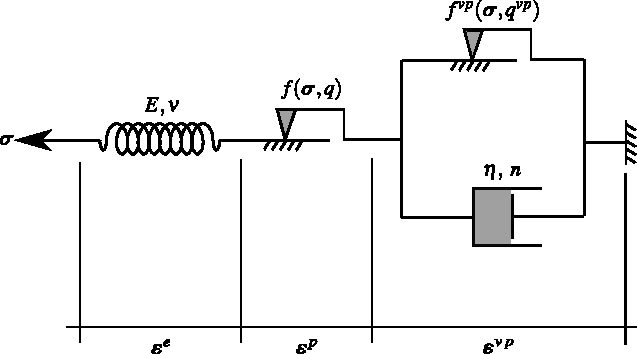
\includegraphics[scale=1]{Rheological representation.pdf}
	\caption{Rheological representation of the elastoplastic-viscoplastic model.}
	\label{reological_scheme}
\end{figure}
\FloatBarrier
In the three-dimensional context, the plasticity component of constitutive behavior is described by a Drucker-Prager plastic flow surface given by:
\begin{equation}
	\label{eq:f_Drucker_Prager}
	f(\stress,q) = f(I_1,J_2,q) = \beta_1 I_1 +\beta_2 \sqrt{J_2}-q(\alpha),
\end{equation}
which $I_1$ is the first invariant of the stress tensor, $J_2$ the second invariant of the deviator tensor and $\beta_1, \beta_2$ and $q(\alpha)$ are strength parameters related to the friction angle $\phi$ and cohesion $c(\alpha)$, respectively. Drucker-Prager plasticity surface inscribed to the Mohr-Coulomb surface shall be considered throughout the subsequent analysis [\citenum{bernaud1991}]:
\begin{equation}
	\label{eq:f_DP_inscrita_MC}
	\beta_1 = \dfrac{(k-1)}{3}, ~~~ \beta_2 = \dfrac{(2k+1)}{\sqrt{3}}, ~~~
	q(\alpha) = 2\sqrt{k}~c(\alpha),
\end{equation}
where $k = (1+\sin{\phi})/(1-\sin{\phi})$. The internal variable $\alpha$ is the equivalent plastic strain $\straineqp$ used to simulate strain hardening/softening phenomena. However, for this study, we adopt perfect plasticity, meaning that c is a constant. For the viscoplasticity surface $f^{vp}$ the same surface is employed, but with $\phi^{vp}$ in $\beta_1$ and $\beta_2$, and $q^{vp} = 2\sqrt{k^{vp}}-c^{vp}$ where $k^{vp} = (1+\sin{\phi^{vp}})/(1-\sin{\phi^{vp}})$ and $c^{vp}$ is a constant, i.e., perfect viscoplasticity. 
The plastic flow rule is given by:
\begin{equation}
	\label{eq_plastic_flow}
	\dot \strainp = \left\{ 
	\begin{array}{ll} 
		\dot \lambda \dfrac{\partial g}{\partial \stress} &  \text{for } f > 0 \\ 
		\zerol, & \text{for } f \le 0 \\
	\end{array}\right.,
\end{equation}
where $\dot \lambda$ is the plasticity multiplier and $g$ is a potential flow function analogous to $f$ used to simulate the volume dilatation during the evolution of plastic deformations. However, for this analysis, was used associated plasticity, i.e., $g=f$. The plastic multiplier is obtained through the consistency condition $\dot f = 0$. Numerical details of this implementation can be found in [\citenum{quevedo2022b}]. For viscoplastic flow rule we have,
\begin{equation}
	\label{eq_viscoplastic_flow}
	\dstrainv = \dot \lambda^{vp} \dfrac{\partial f^{vp}}{\partial \stress}
\end{equation}
In contrast to the plastic multiplier, the viscoplastic multiplier $\lambda^{vp}$ is independent of a consistency like condition. As a result, its expression is explicit. Based on the framework of generalized Perzyna's overstress theory [\citenum{perzyna1966}], its expression may be derived as follows:
\begin{equation} \label{eq_perzyna_model}
	\dot \lambda^{vp} = \dfrac{\Phi(\stress,q^{vp})}{\eta}~~~\text{and}~~~\Phi = \left\langle  \dfrac{f^{vp}(\stress,q^{vp})}{f_0} \right\rangle^n, \,
\end{equation} where $\Phi$ is the overstress function, $\eta$ is the dynamic viscosity constant, $n$ is the dimensionless parameter that gives the form of the power law, $f_0$ a parameter conveniently adopted and $\left\langle * \right\rangle$ is the McCauley function which is $0$ when $* <0$ , i.e. viscoplastic flow will only occur when the overstress function is positive.

In this coupled model, when $\phi=\phi^{vp}$, cohesion entirely controls the evolution of local mechanical fields. Specifically, when  $c \rightarrow \infty$ and $c^{vp} \rightarrow \infty$, the system achieves a purely elastic solution. The solution becomes purely elastoviscoplastic with $c \rightarrow \infty$, while a pure elastoplastic solution emerges with $c^{vp} \rightarrow \infty$. In the coupled analysis, condition $c^{vp} < c$ is adopted, allowing the viscoplastic domain to occur without plasticity. However, in the presence of plasticity, viscous effects become inevitable. Fig.~\ref{epvpdomains} illustrates these domains in principal stress space.
\begin{figure}[h!]
	\centering
	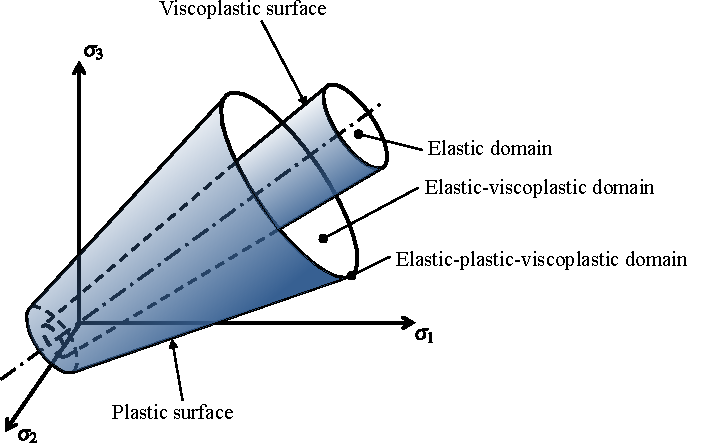
\includegraphics[scale=0.8]{Elastic-plastic-viscoplastic domains.pdf}
	\caption{Elastoplastic-viscoplastic domains.}
	\label{epvpdomains}
\end{figure}

\section{Constitutive Model of the Lining}\label{sec4}

Shrinkage and creep phenomena represent fundamental components of concrete deformation processes that are expected to naturally affect the instantaneous as well as the transient and long-term behavior of structures involving such material. However, most of the tunnel design analyses consider the concrete involved in lining systems as a linear elastic material. From a phenomenological point of view, creep of concrete refers to the time-dependent deformation induced by sustained loading, whereas shrinkage deformation refers to the volume decrease caused by drying. As far as deformation in tunnel structures is concerned, creep and shrinkage have an important effect on the performance of the concrete lining and consequently on its contribution to controlling the long-term convergence of the tunnel. To account for such constitutive features, the concrete creep deformation is addressed by means of an aging viscoelastic rheological model relying on Bažant and Prasannan Solidification Theory [\citenum{bazant:1989a},  \citenum{bazant:1989b}]. The viscoelastic model is described by a Generalized Kelvin-chain as depicted in Fig.~\ref{reological_representation_concrete}. The mechanical parameters that define such a rheological model are the springs stifness and dash-pots viscosity. The model parameters are calibrated based on the CEB-FIP MC90 standard specifications formulation reported in [\citenum{CEB:1993}]. One may refer to [\citenum{quevedo2018} , \citenum{quevedo2022}] for detailed description of the calibration procedure. As regards the concrete deformation associated with shrinkage, the isotropic formulation proposed in CEB-FIP MC90 standard [\citenum{CEB:1993}] is adopted in the present modeling and subsequent computational analyses. Full details regarding model definition and related finite element implementation may be found in [\citenum{quevedo2017comportamento}] and [\citenum{quevedo2022}].

\begin{figure}[h!]
	\centering
	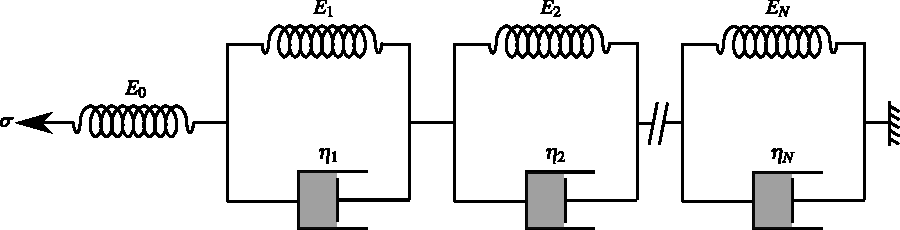
\includegraphics[scale=1]{Rheological_representation_concrete.pdf}
	\caption{Generalized Kelvin model for uniaxial concrete viscoelasticity.}
	\label{reological_representation_concrete}
\end{figure}

Accordingly, the constitutive equations for concrete lining relating the stress and strain rate can be expressed in the framework of infinitesimal strain analysis as:
\begin{equation} \label{eq:8}
	\dstress = \Dll : \dstraine = \Dll : \dstrain - \Dll : \dstrainsh - \Dllmod : \dstraincr\;
\end{equation}

In the above relationship, $\dstrainsh$  and $\dstraincr$ are respectively the shrinkage and creep strain rates. The fourth-order tensors $\Dll$ and $\Dllmod$ refer to the isotropic elastic linear constitutive tensor and modified constitutive tensor that incorporate the aging viscoelastic properties of the concrete, respectively.

For the numerical implementation purposes, relationship (\ref{eq:8}) may conveniently be written in incremental form: 
\begin{equation} \label{eq:9}
	\Delta \stress = \Dll : \Delta \strain - \Dll : \Delta \strainsh - \Dllmod : \Delta \straincr \;
\end{equation}

As mentioned above, isotropic formulation is considered for shrinkage, so that increment of shrinkage strain reads:
\begin{equation} \label{eq:10}
	\Delta \strainsh =  \Delta \strainshCEB(t_{s}) \onell \;
\end{equation}
where $t_{s}$ represents the concrete curing time, and $\Delta \strainshCEB$ is the variation in magnitude of the concrete deformation associated with shrinkage (the dependency $\Delta \strainshCEB$ of on current time is omitted). The latter expression is determined based on CEB-FIP MC90 standard specifications [\citenum{CEB:1993}]. 

Regarding the increment of creep strain $\Delta \straincr$, its value is computed making use of the incremental algorithm developed by Bažant and Prasannan [\citenum{bazant:1989a,bazant:1989b}], together with a model calibration that incorporates CEB-FIP MC90 standard formulation [\citenum{CEB:1993}]. More precisely, the three-dimensional ageing viscoelastic behavior of isotropic concrete is defined by the Generalized Kelvin model for the relaxation modulus under uniaxial stress, whereas the Poisson ratio is assumed to be time independent within the time interval of analysis. The procedure for the identification of model parameters is achieved by comparing the creep functions provided in references [\citenum{bazant:1989a,bazant:1989b}] and [\citenum{CEB:1993}], leading to the following equivalence:
\begin{equation} \label{eq:11}
	E_0 = E_c(t_0),~ \gamma(t-t_0)=\beta_c(t-t_0),~ \frac{1}{v(t)} = \frac{\phi_0(t_0)}{E_{ci}} \text{  and  } \frac{1}{\eta(t)} \to 0 \;
\end{equation}
in which $t$ refers to the current time value and $t_0$ to the concrete age at the instant of load application (time interval $t-t_0$ is generally referred to as loading time or loading age). In the Generalized Kelvin model introduced by Bažant and Prasannan [\citenum{bazant:1989a,bazant:1989b}], $E_0$ is the instantaneous elasticity modulus of the concrete formed aggregates and cement paste particles, $\gamma(t-t_0) = \sum\limits_{i=1}^{N}\gamma_i$ is the microviscoelastic deformation of the volume fraction $v(t)$ of solidified concrete and $\eta(t)$ is the apparent macroscopic viscosity. In the CEB-FIP MC90 formulation [\citenum{CEB:1993}], $E_c(t_0)$ stands for the tangent elastic modulus of concrete at the instant of the loading application $t_0$, $\beta_c(t-t_0)$ is a coefficient that depends on the loading age $t-t_0$, $\phi_0(t_0)$ is a coefficient defining the delayed strain when loaded at age $t_0$ of the concrete, and $E_{ci}$ represents the tangent elasticity modulus of the concrete at the age of $28$ day.

\section{Spatial and time discretization of the domain}\label{section_spatial}

The geometry model of analyzed domain $\Omega$ is schematically displayed in Fig.~\ref{domain}. It consists of a system of deep twin tunnels connected with a transverse gallery. The radius of the circular longitudinal tunnels is denoted by $R_t$, whereas that of the circular connecting gallery is denoted by $R_g \le R_t$. The underground structure is excavated in a homogeneous rock mass at great depth $H \gg R_t$.
\begin{figure}[h!]
	\centering
	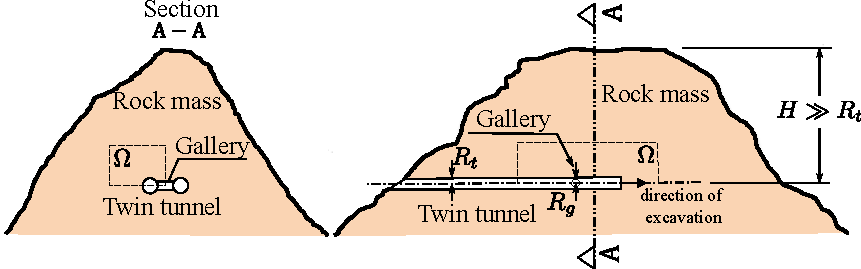
\includegraphics[scale=1]{Domain.pdf}
	\caption{Schematic representation of the twin tunnels geometry problem.}
	\label{domain}
\end{figure}
\FloatBarrier
Within the analyzed material domain, the initial stress state prevailing in the rock mass prior to the tunnel excavation process is defined by constant vertical and horizontal geostatic stress $\sigma_v$ and $\sigma_h$, taking the following form:
\begin{equation} \label{eq:stress0}
	\stress_0 = -\sigma_v \ey \otimes \ey - \sigma_h\left( \onell - \ey \otimes \ey \right)
\end{equation}

where is the upward unit vector parallel to vertical direction. The initial horizontal stress is generally related to the vertical stress by means of the horizontal thrust coefficient $\sigma_h = k_0 \sigma_v$. Starting from the initial configuration of the material system $\Omega$, the processes of excavation (advancing face) and lining placement are simulated by means of the “activation/deactivation” technique [\citenum{bernaud1995}, \citenum{bernaud2009}, \citenum{maghous2012}, \citenum{quevedo2022}].


The geometry material domain $\Omega$ considered for the finite element simulations, including tunnelling and deformation analysis, is defined by a parallelepiped volume of dimensions $\left(L_1+L_2 \right ) \times L_3 \times d_3$ (Fig. 5). Owing to the symmetry of the problem, only the material domain $\left\{x \le 0, y \ge 0\right\}$   is considered for F.E discretization and analysis. Referring to the notations of Fig.~\ref{Mesh1}, $d_1$ is the distance between the axes of longitudinal tunnels, $L_2$  represents the total length  along longitudinal direction $\ez$ of the cylindrical  volume to be excavated that is  considered in the numerical simulation, $d_3$ is the thickness along vertical direction $\ey$ of material domain $\Omega$, $L_1$ stands for the length of unexcavated region after total excavation process, $L_3$ is the total length along transversal direction $\ex$ of discretized material domain, $d_2$ characterizes the location of the circular transverse axis gallery that intersects the  longitudinal tunnel at $z = L_1+d_2$. The length of the excavation step adopted  will be denoted by $L_{pt}$. The finite element model including geometrical discretization and boundary conditions is illustrated in Fig.~\ref{Mesh1}. The mesh used in the simulations consists of $119740$, $182470$ or $221104$ total elements (hexahedra and tetrahedra), depending on the value of spacing between longitudinal tunnels. To increase the accuracy of the model predictions in the intersection zone, the region surrounding the transverse gallery (including part of the longitudinal tunnel) is discretized by means 10-node quadratic tetrahedral elements, whereas 8-node trilinear hexahedral elements are used for the remaining part of the structure.   Furthermore, a refined meshing is used for discretizing the zones surrounding the longitudinal and transverse gallery. These zones whose mechanical state is significantly affected by the tunnelling process are indicated by light gray color in Fig.~\ref{Mesh1}.
\begin{figure}[h!]
	\centering
	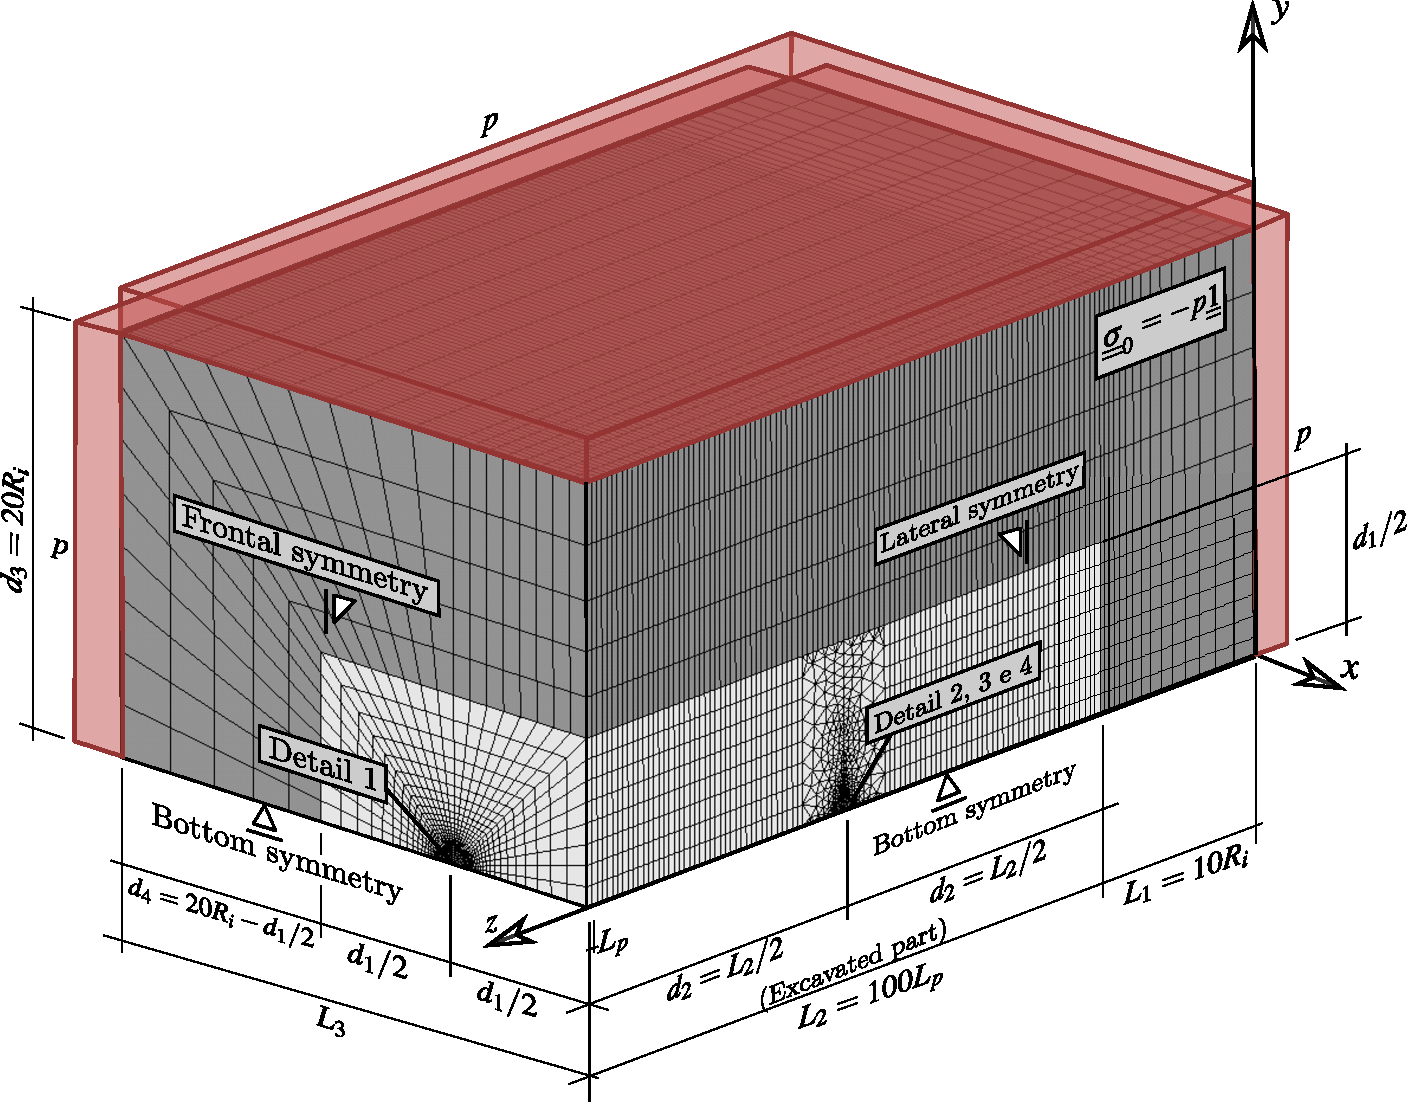
\includegraphics[scale=0.5]{Mesh1.pdf}
	\caption{Mesh, dimensions and boundary conditions of the 3D twin tunnel domain.}
	\label{Mesh1}
\end{figure}

Figures \ref{Mesh2} to \ref{Mesh6} display some details regarding the geometry and F.E discretization of the structure. Fig.~\ref{Mesh2} presents some details of the longitudinal tunnel cross-section in a $xy$ plane, together with the layer of concrete lining (in sky blue color), parameter $e_t$ being the thickness of the lining. Installation of the lining (shotcrete or precast concrete) is simulated in the F.E modeling by progressive activation of the corresponding elements, which consists in assigning to these elements the concrete mechanical properties.
\begin{figure}[h!]
	\centering
	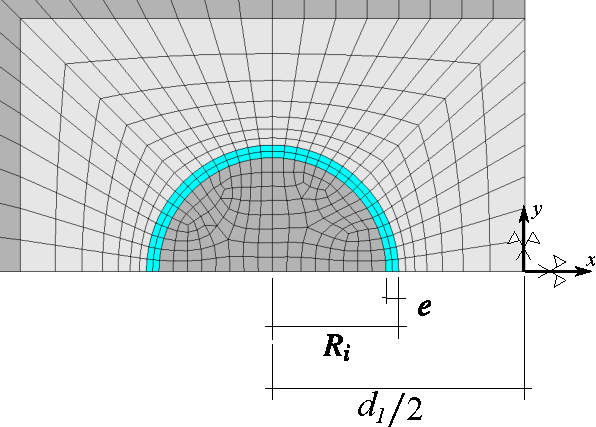
\includegraphics[scale=0.8]{Mesh2.pdf}
	\caption{Detail 1 - Mesh in longitudinal tunnel cross-section with spacing $d_1=4R_t$.}
	\label{Mesh2}
\end{figure}
\FloatBarrier

An important issue investigated in this work is the influence of the spacing $d_1$ between twin tunnels on their convergence. Fig.~\ref{Mesh3} and Fig.~\ref{Mesh4} illustrate the spatial discretization of the gallery region as well as of the connection with the longitudinal tunnel. Three values shall be considered for the spacing $d_1$ in the numerical simulations, namely  $d_1 = 16R_t, 8R_t$ and $4R_t$. The layer of concrete lining of thickness $e_g$ installed along the gallery wall is indicated by red color in the figures. Without introducing additional modeling restriction and for the sake of simplicity, the value of the gallery radius is fixed to $R_g = 2/3R_t$. The same lining system (same concrete material and layer thickness) is considered for both longitudinal tunnels and gallery. As regards the discretization of the region surrounding the gallery, parameters $d_5$ and $d_1$ define the size in a $yz$ plane of the transition region involving the tetrahedral finite elements. Fig.~\ref{Mesh5} provides a view of the transition region and tunnel/gallery intersection zone.
\begin{figure}[h!]
	\centering
	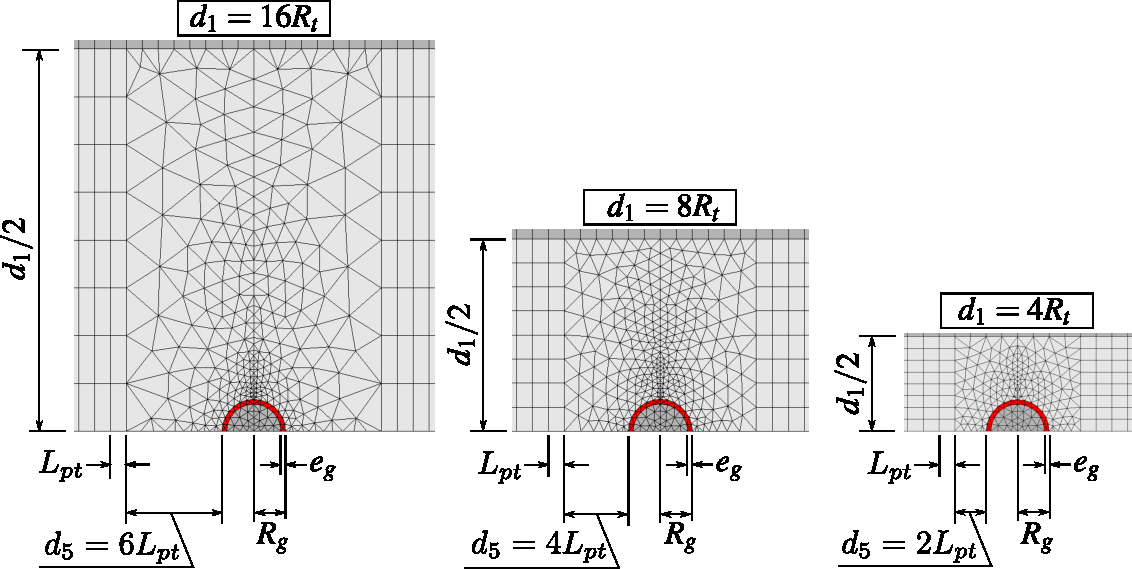
\includegraphics[scale=0.8]{Mesh3.pdf}
	\caption{Geometry and F.E mesh of gallery cross-section for configurations $d_1=16R_t$, $d_1=8R_t$ and $d_1=4R_t$.}
	\label{Mesh3}
\end{figure}
\begin{figure}[h!]
	\centering
	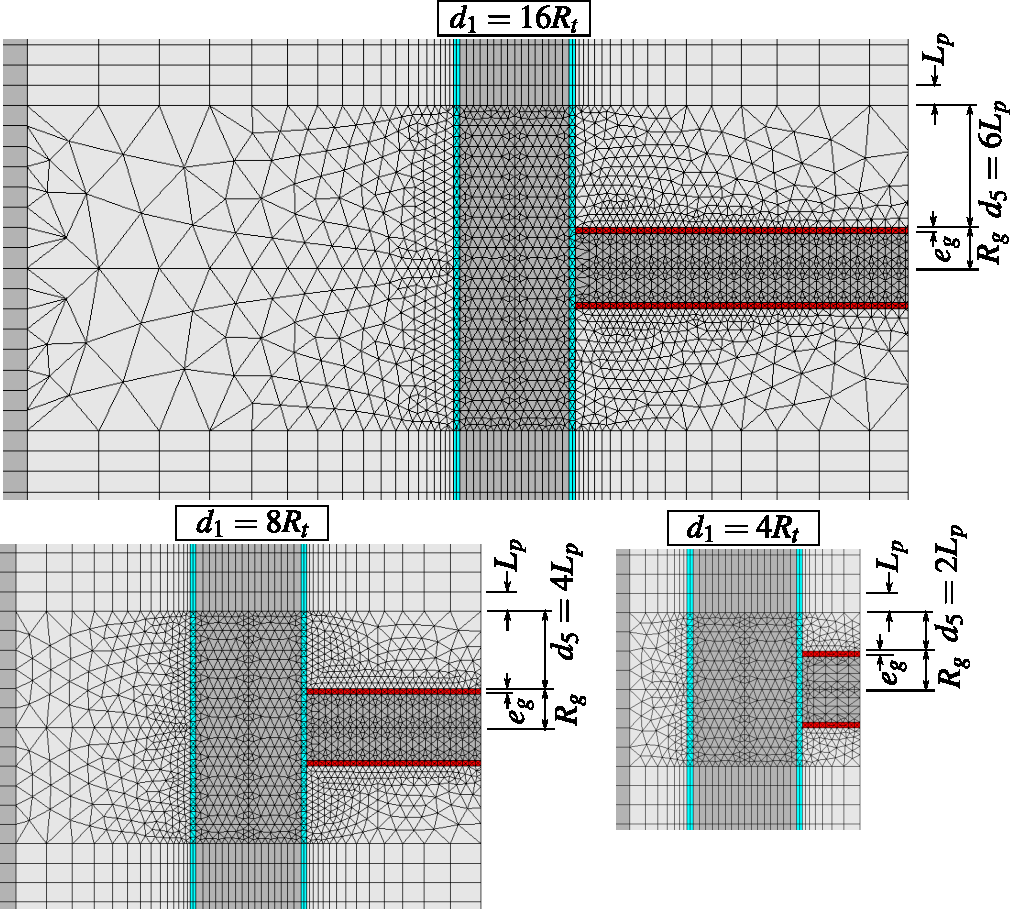
\includegraphics[scale=0.6]{Mesh4.pdf}
	\caption{Views of longitudinal tunnel and gallery in the symmetry plane $y=0$ for configurations $d_1=16R_t$, $d_1=8R_t$ and $d_1=4R_t$.}
	\label{Mesh4}
\end{figure}
\begin{figure}[h!]
	\centering
	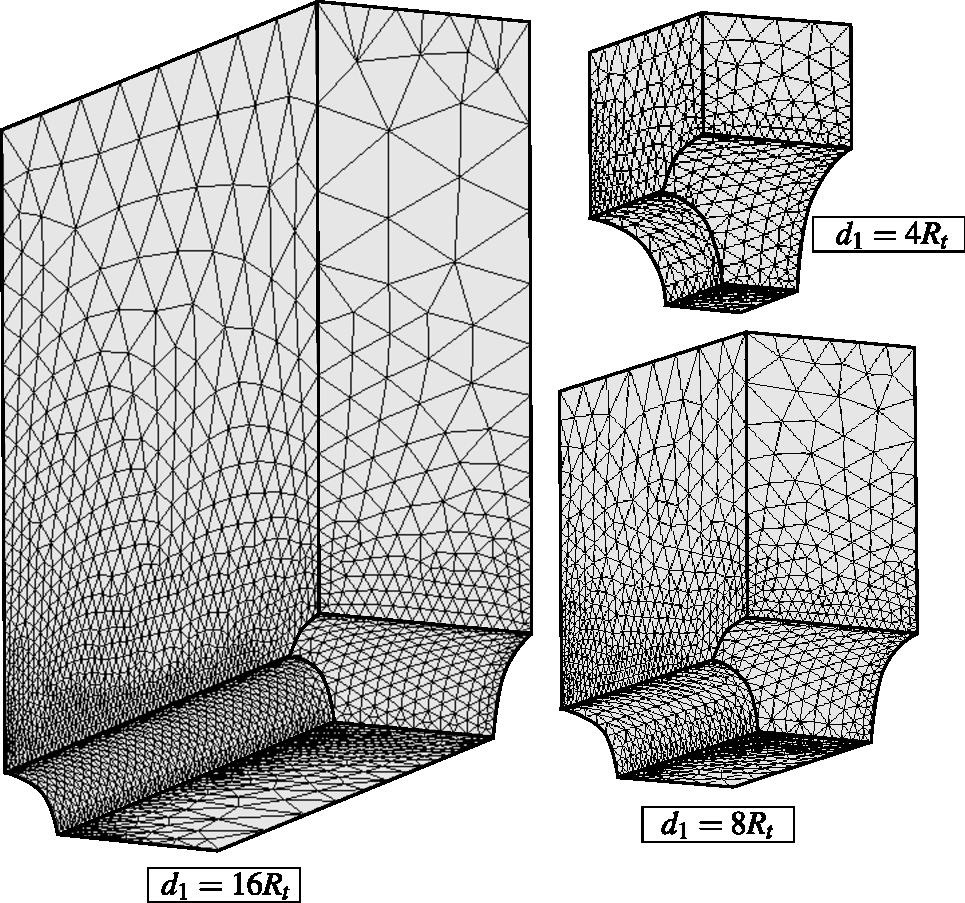
\includegraphics[scale=0.6]{Mesh5.pdf}
	\caption{View of the transition and tunnel/gallery intersection zones for configurations $d_1=16R_t$, $d_1=8R_t$ and $d_1=4R_t$.}
	\label{Mesh5}
\end{figure}
\FloatBarrier

Finally, Fig.~\ref{Mesh6} presents the F.E mesh used for the layer of concrete lining in both the longitudinal layer (in sky blue color) and the gallery (in red color) for the three configurations $d_1=16R_t$, $d_1=8R_t$ and $d_1=4R_t$, with specific details on the junction region of the gallery and the longitudinal tunnel. For the illustration purposes, symmetry with respect to plane $y = 0$ has been used to complete the geometry representation of each configuration. It is emphasized that the tetrahedral elements used for the discretization of the region surrounding the transverse gallery exactly fits excavation steps (elements removal or deactivation).

\begin{figure}[h!]
	\centering
	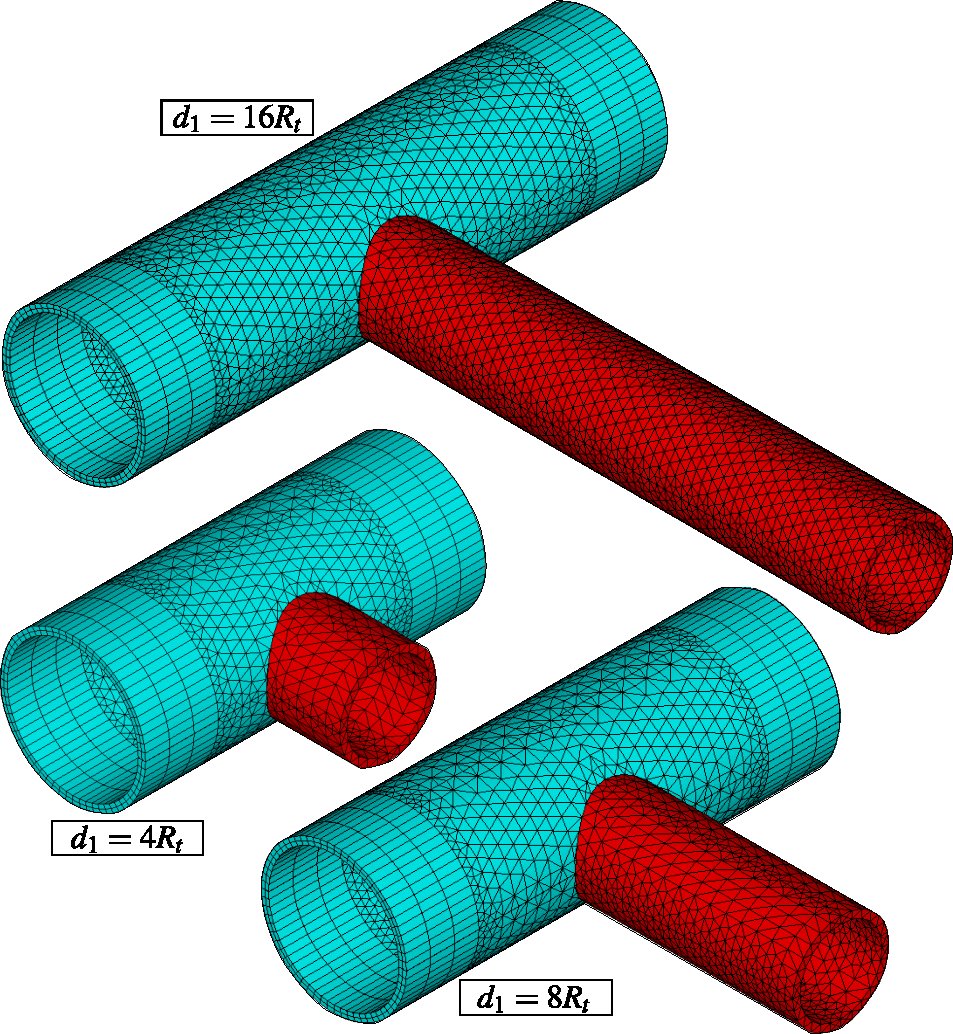
\includegraphics[scale=0.6]{Mesh6.pdf}
	\caption{Isometric view of the lining at the intersection for $d_1=16R_t$, $d_1=8R_t$ and $d_1=4R_t$ - expansion of symmetry in the $xz$ plane.}
	\label{Mesh6}
\end{figure}
\FloatBarrier

As mentioned previously, the tunnelling process, including the excavation steps and lining installation, is simulated resorting to the activation-deactivation method. Each excavation step is modeled by deactivation of the corresponding elements (the elements stiffness is reduced by a factor $1E8$), whereas installation of elements of lining at a distance $d_{0t}$ from the excavation face (unlined length) is achieved through activation of the corresponding elements by assigning them concrete properties. The F.E solution of the time-dependent problem is performed for each excavation step associated with time interval $t_p = L_p/V_p$, where $L_{pt}$ represents the length of the excavation step and $V_{pt}$ is the speed of the excavation face. Fig. 11 schematically displays the consecutive phases of excavation process. In this Figure, $n_p$ is the total number of excavation steps and $n_{pig}$ represents the number of longitudinal tunnel excavation steps prior to gallery excavation. After achievement of the $n_{pig}$ excavation steps, the excavation of the gallery is initiated starting from the longitudinal tunnel wall. Referring to the notation of Fig. 11,  $L_{pg}$ is the considered step length for the gallery excavation, $V_{pg}$ is the speed of the gallery excavation, and $d_{0g}$ is the unlined length of the gallery. Each gallery excavation step is associated with time interval $t_{pg} = V_{pg}/L_{pg}$. After the gallery excavation is completed, we proceed to further excavation steps of the longitudinal tunnel. 

For the sake of clearness, the main parameters defining the geometry domain as well as and excavation process and lining installation are summarized in Table~\ref{table1}. 
\begin{figure}[h!]
	\centering
	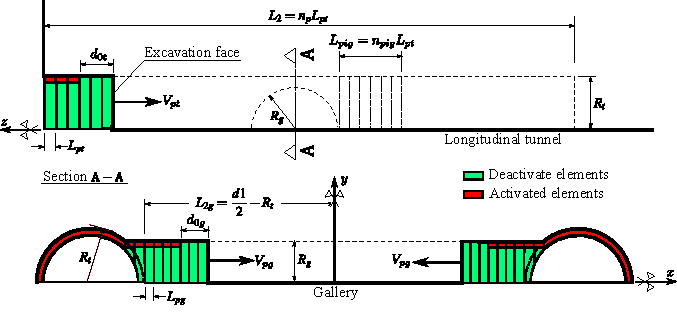
\includegraphics[scale=1.3]{Diagram of excavations.pdf}
	\caption{Schematic representation of the excavation process.}
	\label{Diagram of excavations}
\end{figure}
\FloatBarrier
\begin{table}
	\caption{Parameters related to the geometry of the domain, excavation and installation of the lining.}
	\label{table1}
	\centering
	%\small
	\renewcommand{\arraystretch}{1.25}
	\begin{tabular}{c c c c}
		\hline
		\multicolumn{1}{c}{PARAMETERS} &
		\multicolumn{1}{c}{SYMBOL} &
		\multicolumn{1}{c}{UNIT} &
		\multicolumn{1}{c}{VALUES} \\
		\hline
		\multicolumn{4}{c}{Longitudinal tunnels} \\
		\hline
		Radius of the longitudinal tunnel & $R_t$ & m & $R_t$ \\
		Thickness of the lining & $e_t$ & m & $0.1R_t$ \\
		Step length of the excavation process & $L_{pt}$ & m & $1/3R_t$ \\
		Unlined length & $d_{0t}$ & m & $2L_{pt}$ \\
		Speed of the excavation face & $V_{pt}$ & m/day & $12.5$ \\
		Excavation step time & $t_p$ & day & $L_{pt}/V_{pt}$ \\
		\hline
		\multicolumn{4}{c}{Gallery} \\
		\hline
		Radius of the gallery & $R_{g}$ & m & $2/3R_t$ \\
		Thickness of the concrete lining & $e_g$ & m & $0.1R_t$ \\
		Step length of the excavation process \footnote{1} & $L_{pg}$ & m & $1/3R_g$ \\
		Unlined length & $d_{0g}$ & m & $2L_{pg}$ \\
		Speed of the excavation face & $V_{pg}$ & m/day & $12.5$ \\
		Number of steps that starts gallery excavation & $n_{pig}$ & un & $15$ \\
		\hline
		\multicolumn{4}{c}{Rest of domain} \\
		\hline
		Distance between longitudinal tunnel axes & $d_1$ & m & $4R_t ~8R_t ~16R_t$ \\
		Thickness along vertical direction $\ey$ & $d_3$ & m & $20R_t$ \\
		Length of the unexcavated region & $L_1$ & m & $10R_t$ \\
		Total excavated length & $L_2$ & m & $100L_{pt}$ \\
		Thickness along transversal direction $\ex$ & $L_3$ & m & $20R_t + d_1/2$ \\
		\hline
	\end{tabular}
	\normalsize
	\\ \footnotemark[1]{{\footnotesize Value of $L_{pg}$ is slightly different for the last excavation step to match the gallery lengh.}}
\end{table}
\FloatBarrier
During the tunnel construction phases, the time increment used for the time-dependent analysis is automatically managed by the ANSYS solver. The latter makes use of a semi-implicit scheme for the viscoplasticity solution, together with an automatic time stepping algorithm [\citenum{zienkiewicz1974visco}] in which the time step is defined as a fraction of time $t_p$ for the phases of longitudinal tunnel excavation and as a fraction of $t_{pg}$ for the phases of transverse gallery excavation. Furthermore, distinct time steps are considered for the time-dependent analysis during tunnelling process and post-excavation stage. After complete tunnel construction phases, the analysis is carried out for a period of about $3000$ days to assess the time evolving deformation as well as long-term viscous effects on the final equilibrium of the tunnel structure. At that respect and in anticipation of the numerical results of the subsequent sections, the characteristic viscoplastic relaxation time [\citenum{simo1998}] is equal to $\bar{\tau} = \eta f_0 / E$ , which is close to $30$ days for model data of Table~\ref{table2}.

\section{Preliminary numerical simulations and computational model verification}\label{sec6}

This section is aimed at applying the computational modeling to simulate deformation and stress in two academic twin tunnels configurations. The numerical results provided in these illustrative applications may be viewed as preliminary verifications of the F.E formulation. The first application refers to unlined twin tunnels excavated in an elastic rock mass, whereas the second application addresses the situation of unlined twin tunnels excavated in an elastoplastic medium.

\subsection{Unlined twin tunnels in elastic medium}

In the context of plane strain conditions, Guo et al. [\citenum{GUO2021}] addressed the configuration of deep twin tunnels excavated in a homogeneous elastic medium in which prevails a hydrostatic initial stress distribution. The authors formulated approximate analytical solutions for the stress distribution establishing far behind the face, which are induced in the rock mass by the excavation of two parallel circular tunnels. The model geometry of the twin circular tunnels as well as loading associated with initial hydrostatic stress (i.e., $\sigma_h = \sigma_v$) are displayed in Fig.~\ref{GUO_FIG0}.

Simulation of the problem has been addressed by means of the 3D finite element model and the numerical results obtained for the stress distribution far behind the faces of the twin tunnel shall be compared to the analytical stress solution derived by Guo et al. [\citenum{GUO2021}] in the framework of plane strain conditions. The simulations have been performed taking advantage of symmetry with respect to the midplane between twin tunnels and considering the following model data: tunnel radius $R_t = 4$ m, rock Young modulus $E = 500$ MPa and Poisson ratio $\nu = 0.23$, isotropic initial stresses of $\sigma_v = \sigma_h = 2.2$ MPa.
\begin{figure}[h!]
	\centering
	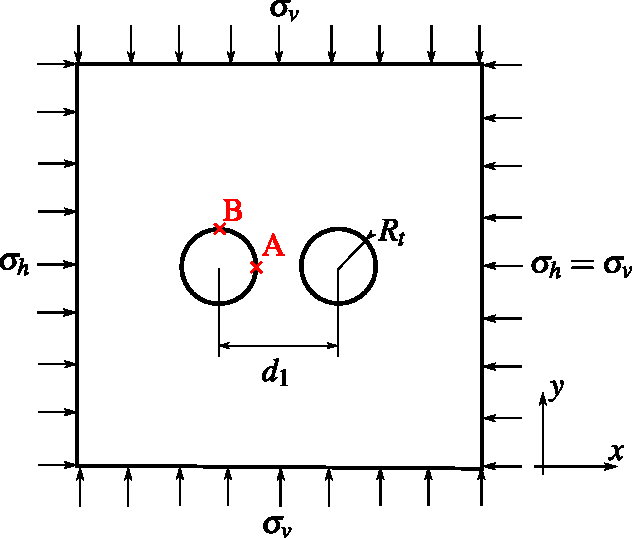
\includegraphics[scale=0.7]{GUO_FIG0.pdf}
	\caption{Geometry model and loading mode of the twin circular tunnels studied in Guo et al. [\citenum{GUO2021}].}
	\label{GUO_FIG0}
\end{figure}
\FloatBarrier

Denoting by $u_y$ the displacement component following the  $y$-axis, Fig.~\ref{Convergence Profiles in B} displays the convergence curves $U_B = -u_y(B)/R_t$ that characterize the inward movement at the tunnel roof $B(x=-d_1/2,y=R_t,z)$ as a function of normalized longitudinal distance to the tunnel face. Several values of normalized distances between the twin tunnels axes $d_1/2R_t$ have been investigated, and the configuration of single tunnel may be viewed as the limiting case $d_1/2R_t \gg 1$. It is recalled that in the latter configuration, the convergence far from the tunnel face that is obtained from an elastic analysis reads $U = \sigma_v(1+\nu)/E$. As expected, this figure indicates that the closer the longitudinal tunnels, the greater the convergence at the roof.
\begin{figure}[h!]
	\centering
	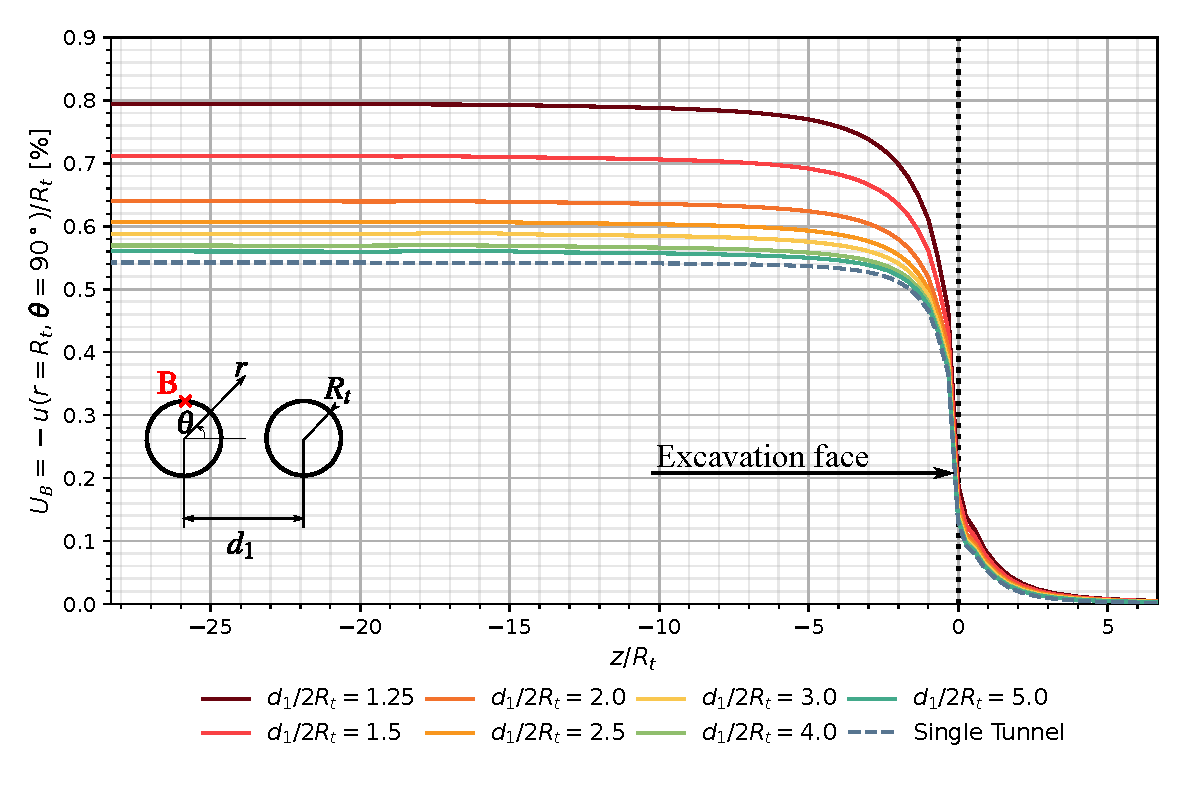
\includegraphics[scale=0.65]{Convergence Profiles in B.pdf}
	\caption{Convergence profiles at the tunnel roof (point B).}
	\label{Convergence Profiles in B}
\end{figure}
\FloatBarrier

The tunnel deformation anisotropy induced by the twin tunnels proximity is illustrated in Fig.~\ref{Relationship between convergence in B and A}, which plots the ratio $U_B/U_A = u_y(B)/u_x(A)$ between the vertical displacement $u_y$ at the roof B and the horizontal displacement $u_x$ at the side wall  $A(x=-d_1/2+R_t, y = 0, z)$. The results shown in this figure refer to a tunnel section located far behind the face at normalized distance $z/R_t = -25$. They emphasize the significative tunnel ovalization induced by the proximity of twin tunnel as the distance $d_1/2R_t$ decreases. 

\begin{figure}[h!]
	\centering
	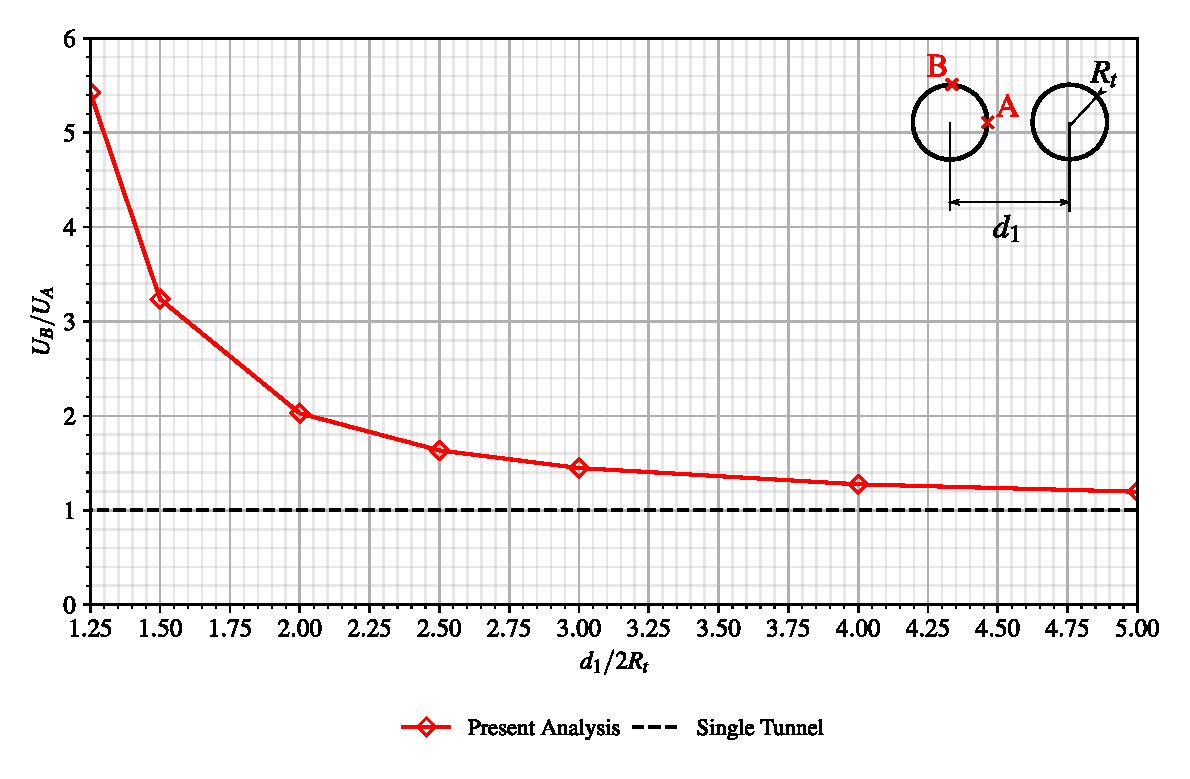
\includegraphics[scale=0.65]{Relationship between Convergence in B and A.pdf}
	\caption{Illustration of the tunnel wall deformation anisotropy induced by twin tunnels proximity.}
	\label{Relationship between convergence in B and A}
\end{figure}
\FloatBarrier

The stress distribution prevailing far from the tunnel face that were obtained from the 3D numerical simulations are compared in Fig.~\ref{Tangencial stress concentration factor in A} to the stress solutions derived analytically and numerically in Guo et al. [\citenum{GUO2021}]. In this figure, the tangential stress concentration factor $\sigma_{yy}/\sigma_v$ computed at the side wall $A$ is plotted for several values of the normalized twin tunnels distance. The results of the theoretical solution to a plate containing two circular holes of equal size presented in Ling et al. [\citenum{ling1948}] are also reported in Fig.~\ref{Tangencial stress concentration factor in A}. It is observed that the results of the 3D finite element simulations correspond to a tunnel section located at normalized distance $z/R_t = -25$ from the face, which is considered sufficient for the plane strain conditions to establish. Interestingly, the tangential stress concentration obtained for a deep single tunnel under plane strain condition simply reads $\sigma_{yy}/\sigma_v = 2$. Although the overall agreement observed between the different predictions, it appears from the comparison that the approximate analytical stress solution provided in [\citenum{GUO2021}] slightly overestimates the tangential stress computed at point A as the value of distance $d_1/2R_t$  increases.

\begin{figure}[h!]
	\centering
	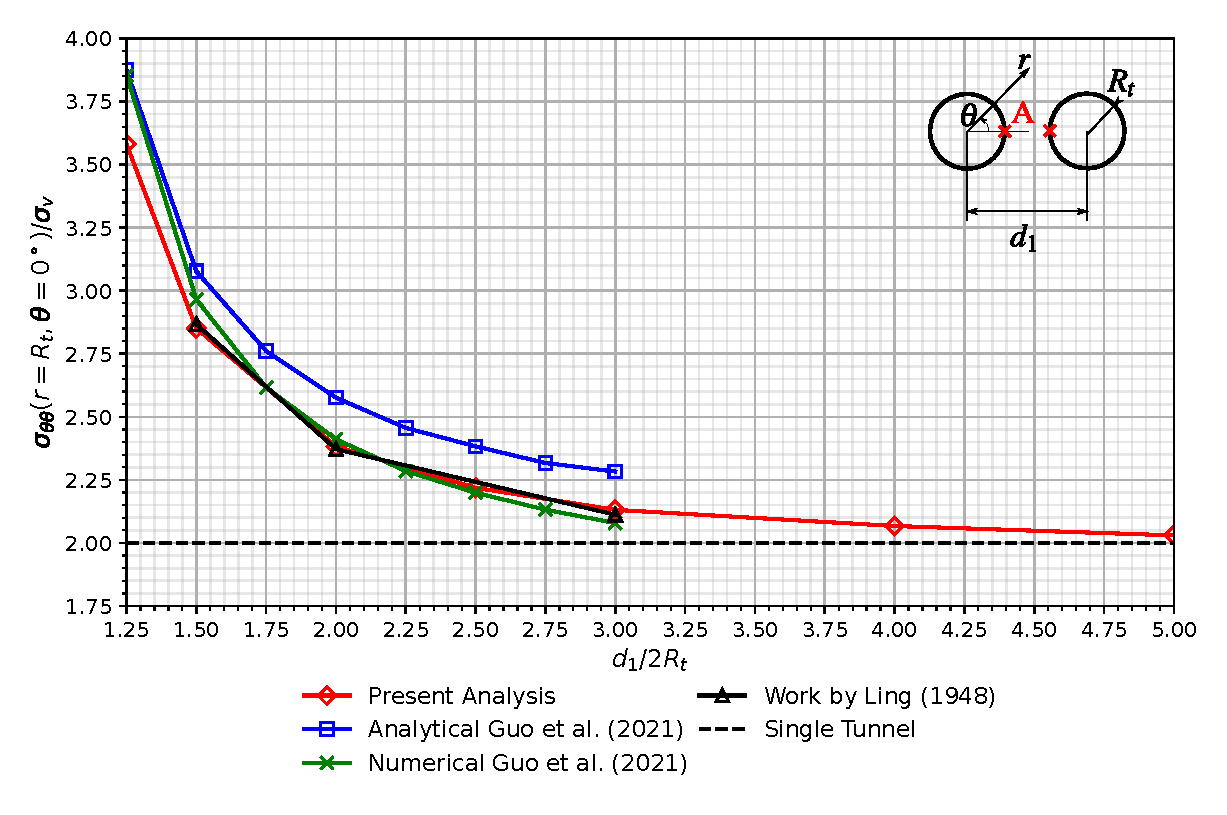
\includegraphics[scale=0.65]{Tangencial stress concentration factor in A.pdf}
	\caption{Tangential stress concentration factor at the side wall A versus twin tunnels distance $d_1/2R_t$.}
	\label{Tangencial stress concentration factor in A}
\end{figure}
\FloatBarrier

Finally, Fig.~\ref{GUO_FIG1} displays the distribution of tangential (orthoradial) stress $\sigma_{\theta \theta}$ around the tunnel boundary $\left\{r = R_t, 0 \le \theta \le \pi\right\}$ considering $d_1/2R_t = 1.5$. The predictions of stress component $\sigma_{\theta \theta}$ obtained from the 3D finite element simulations far behind the tunnel face are shown together with the strain plane solutions derived analytically in [\citenum{GUO2021}], emphasizing the ability of the computational model to accurately capture the effect of tunnels proximity on stress distribution.

\begin{figure}[h!]
	\centering
	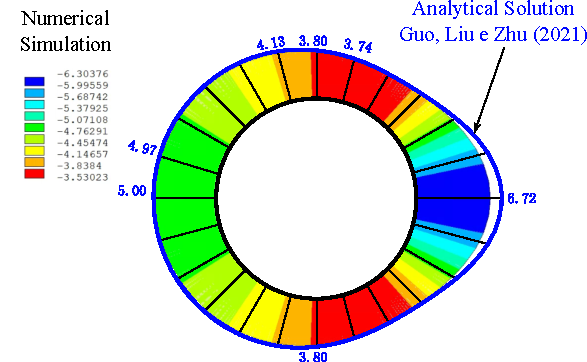
\includegraphics[scale=1]{GUO_FIG1.pdf}
	\caption{Distribution of tangential stress $\sigma_{\theta \theta}$ around the tunnel wall  prevailing far behind the tunnel face (twin tunnels distance $d_1/2R_t = 1.5$).}
	\label{GUO_FIG1}
\end{figure}
\FloatBarrier
Keeping in mind it addresses only an academic configuration, the results provided in this section may be viewed as a first preliminary verification of the accuracy of the computational model formulated for the mechanical interaction in deep twin tunnels.

\subsection{Unlined twin tunnels in elastoplastic medium}\label{}


In the analysis developed by Ma et al. [\citenum{MA2020}], an approximate analytical solution has been formulated for the stresses and the plastic zone boundary around deep twin circular tunnels excavated in a homogeneous elastoplastic medium. The approach carried out under the assumption of plane strain condition makes use of the conformal transformation in the complex variable method to transform the solution of the elastic-plastic interfaces into the determination of the mapping function coefficients.

The geometry model and boundary loading conditions associated with the initial stress state are the same as depicted Fig.~\ref{GUO_FIG0}. Unlike the configuration studied in the preceding section, anisotropic initial stress distributions defined by $\sigma_h \neq \sigma_v$ shall be considered in the present analysis. As regards the rock constitutive model, an elastic-perfectly plastic behavior defined by a Mohr-Coulomb criterion with associated plastic flow rule has been adopted in the study.  Furthermore, the formulation of stress solution for twin tunnels configuration was based on the premise that the plastic zone around each tunnel completely encloses the tunnel edge and the two plastic zones are not connected.

For the comparison purposes, numerical simulations are carried out by means of the 3D finite element model with the aim to investigate the effect of twin tunnels proximity on the tunnel wall deformation. The following model data has been considered in the F.E simulations: tunnel radius $R_t = 1$ m, rock Young modulus $E = 20$ GPa, Poisson ratio $\nu =$ 0.3, friction angle $\phi = 30^\circ$, cohesion $c = 5$ MPa or $2.5$ MPa, initial vertical stress $\sigma_v =30$ MPa or $40$ MPa, initial horizontal stress $\sigma_h = 30$ MPa or $40$ MPa. The simulation took advantage symmetry with respect to the midplane between the twin tunnels has been used for in the F.E discretization model.

Similarly to the analysis developed in the preceding section, the convergence curves $U_B=-u_y(B)/R_t$, which reflects the inward movement at the tunnel roof $B(x=-d_1/2, y=R_t, z)$, is depicted in Fig.~\ref{MA_convergence_profile_B} as a function of normalized longitudinal distance to the tunnel face. Several values of normalized distances between the twin tunnels axes $d_1/2R_t$ have been investigated, together with the reference configuration of single tunnel, the latter being viewed as the limiting case $d_1/2R_t \gg 1$. As it could be expected from such simulations, this figure indicates that the proximity of tunnels significantly increases the convergence at the tunnel roof for small values, say $d_1/2R_t < 2$, of twin tunnel spacing. However, this effect rapidly become negligible as soon as the tunnel spacing increases.

\begin{figure}[h!]
	\centering
	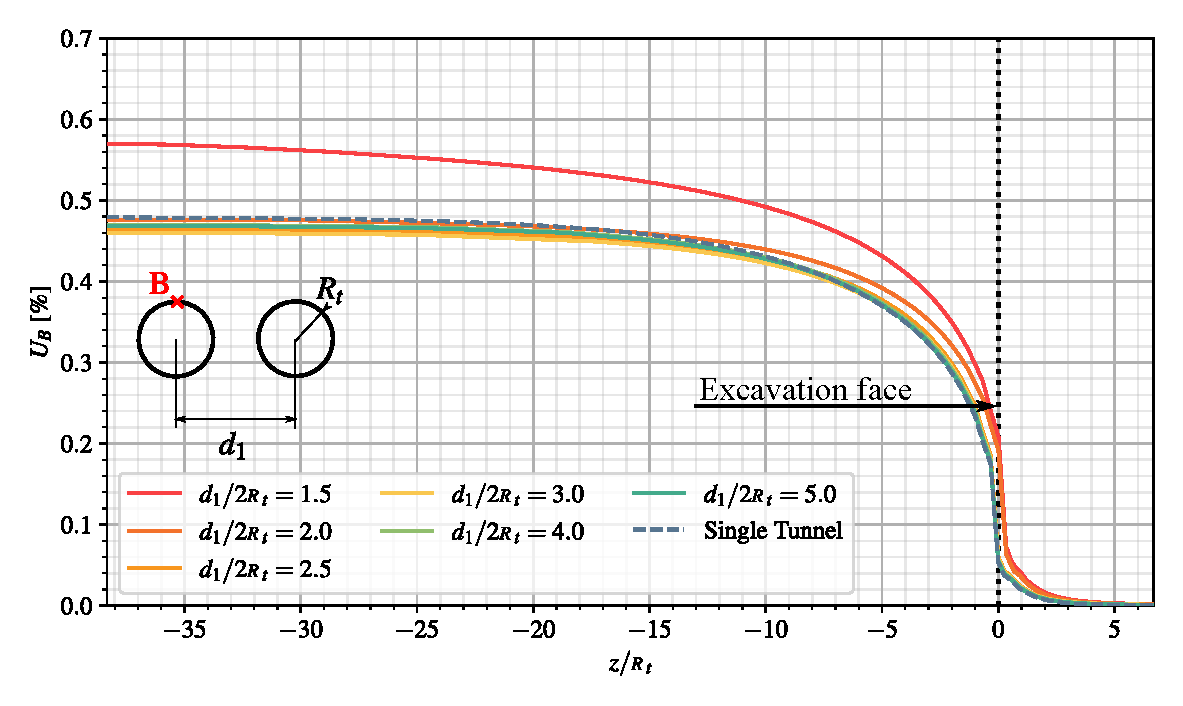
\includegraphics[scale=0.65]{MA_Convergence Profiles in B.pdf}
	\caption{Convergence profiles at the tunnel roof (point B): $c=5$ MPa, $\sigma_v = \sigma_h = 30$ MPa.}
	\label{MA_convergence_profile_B}
\end{figure}
\FloatBarrier

An important feature of the twin tunnels deformation is related to the anisotropy induced by the mutual interaction as the normalized tunnel spacing $d_1/2R_t$ decreases. In that respect, anisotropy of tunnel deformation is illustrated in Fig.~\ref{MA_Relationship between convergence in B and A}, which presents the variations of the ratio $U_B/U_A = u_y(B)/u_x(A)$ between the vertical displacement $u_y$ at the roof $B$ and the horizontal displacement $u_x$ at the side wall $A(x =-d_1/2+R_t, y = 0, z)$ as a function of  normalized twin tunnel spacing $d_1/2R_t$. These results refer to a tunnel section located far behind the face at normalized distance $z/R_t = -35$. As observed in the elastic case studied in the preceding section, the proximity of twin tunnels reflected by small values of normalized distance $d_1/2R_t$ is responsible for tunnel ovalization. The magnitude of horizontal displacement at the side wall $A$ is actually larger in than that of vertical displacement at the tunnel roof $B$, thus indicating an ovalization in the vertical direction (i.e., parallel to $y$-axis).

\begin{figure}[h!]
	\centering
	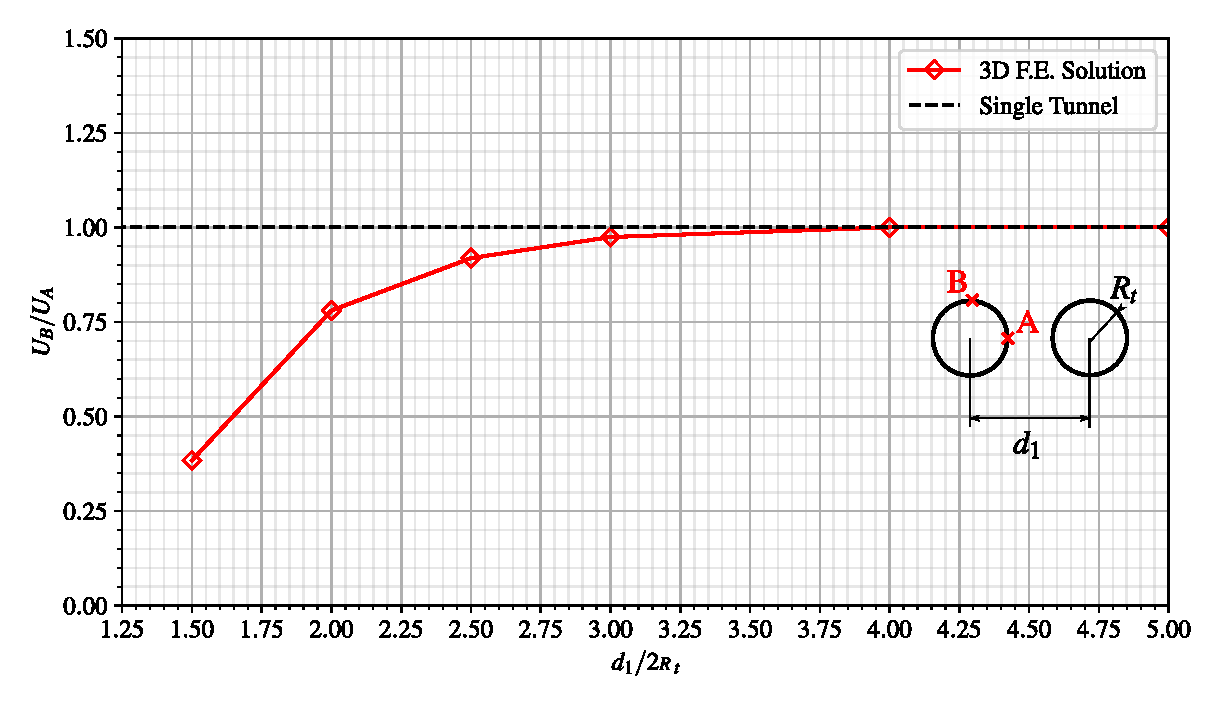
\includegraphics[scale=0.65]{MA_Relationship between Convergence in B and A.pdf}
	\caption{Tunnel wall deformation anisotropy induced by twin tunnels proximity: $c=5$ MPa, $\sigma_v = \sigma_h = 30$ MPa.}
	\label{MA_Relationship between convergence in B and A}
\end{figure}
\FloatBarrier

The stress distribution prevailing far from the tunnel face that were obtained from the 3D numerical simulations are compared in the to the approximate stress solutions derived by Ma et al. [\citenum{MA2020}] within the context of plane strain conditions. Fig.~\ref{MA_FIG1} displays such a comparison in terms of predicted plastic zone surrounding the twin tunnels considering a normalized tunnel spacing of $d_1/2R_t = 2.5$.  Different values have been considered for rock cohesion $c$ and initial stresses $\sigma_v$ and $\sigma_h$. It appears from the latter figure that the finite element modeling produces predictions very similar to those provided in \ref{MA_FIG1}. The results also illustrate that larger plastic zones arise when the cohesion $c$ is smaller.

\begin{figure}[h!]
	\centering
	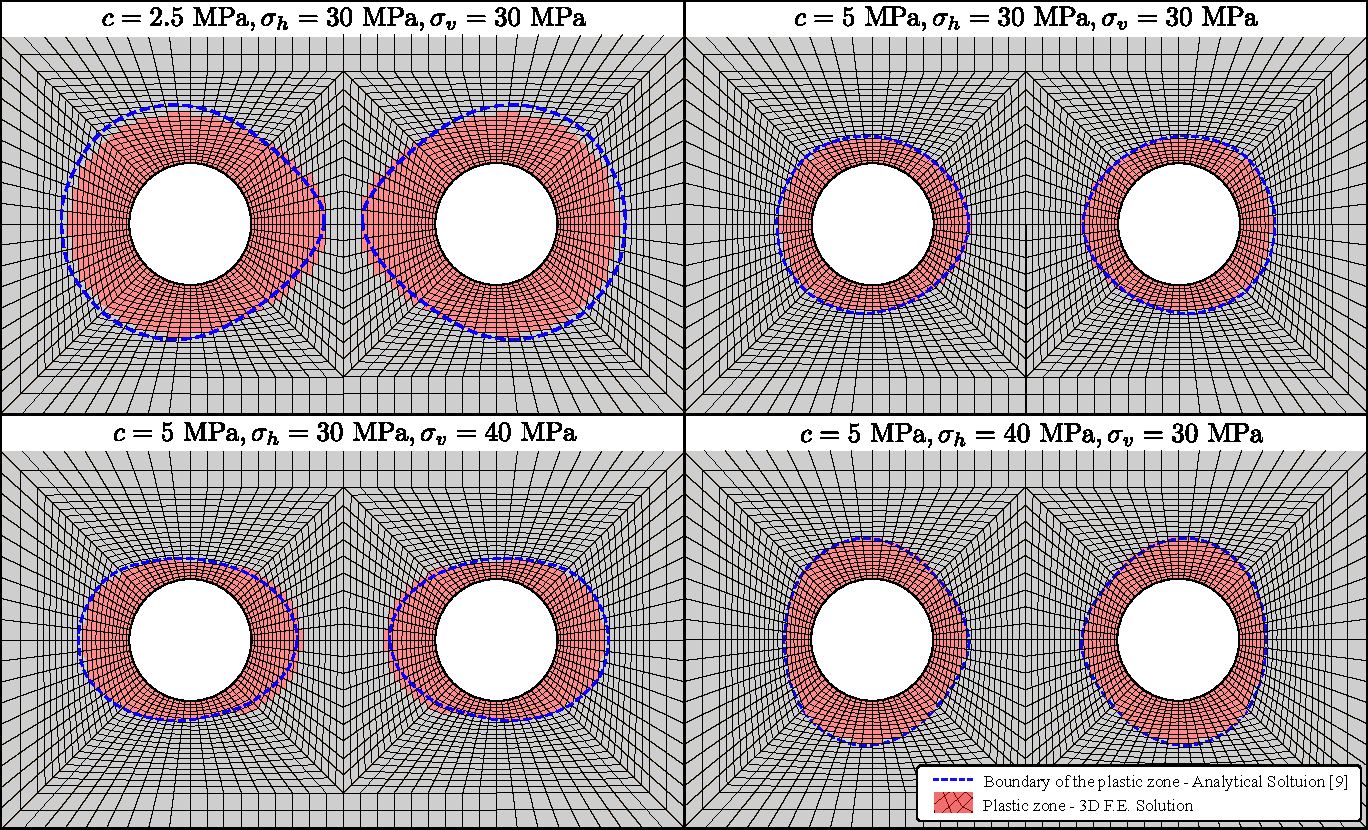
\includegraphics[scale=0.7]{MA_Comparisions_plastic_zones.pdf}
	\caption{The plastic zone extent obtained from the present F.E. simulations and from the stress solution provided in [\citenum{MA2020}].}
	\label{MA_FIG1}
\end{figure}
\FloatBarrier
Further comparisons are shown in Fig.~\ref{MA_stresspaths}, which presents the plots of radial $\sigma_{rr}$, and orthoradial $\sigma_{\theta \theta}$ stress components along three radial paths defined in polar coordinates by $\theta = 45^\circ,~90^\circ \text{~and~} 135^\circ$. It should be pointed out that, although the F.E element simulations make use of the Drucker-Prager yield surface inscribed to the Mohr-Coulomb one (used in the solution of Ma et al. \citenum{MA2020}), the numerical predictions are matching well with the analytical stress solution.

\begin{figure}[h!]
	\centering
	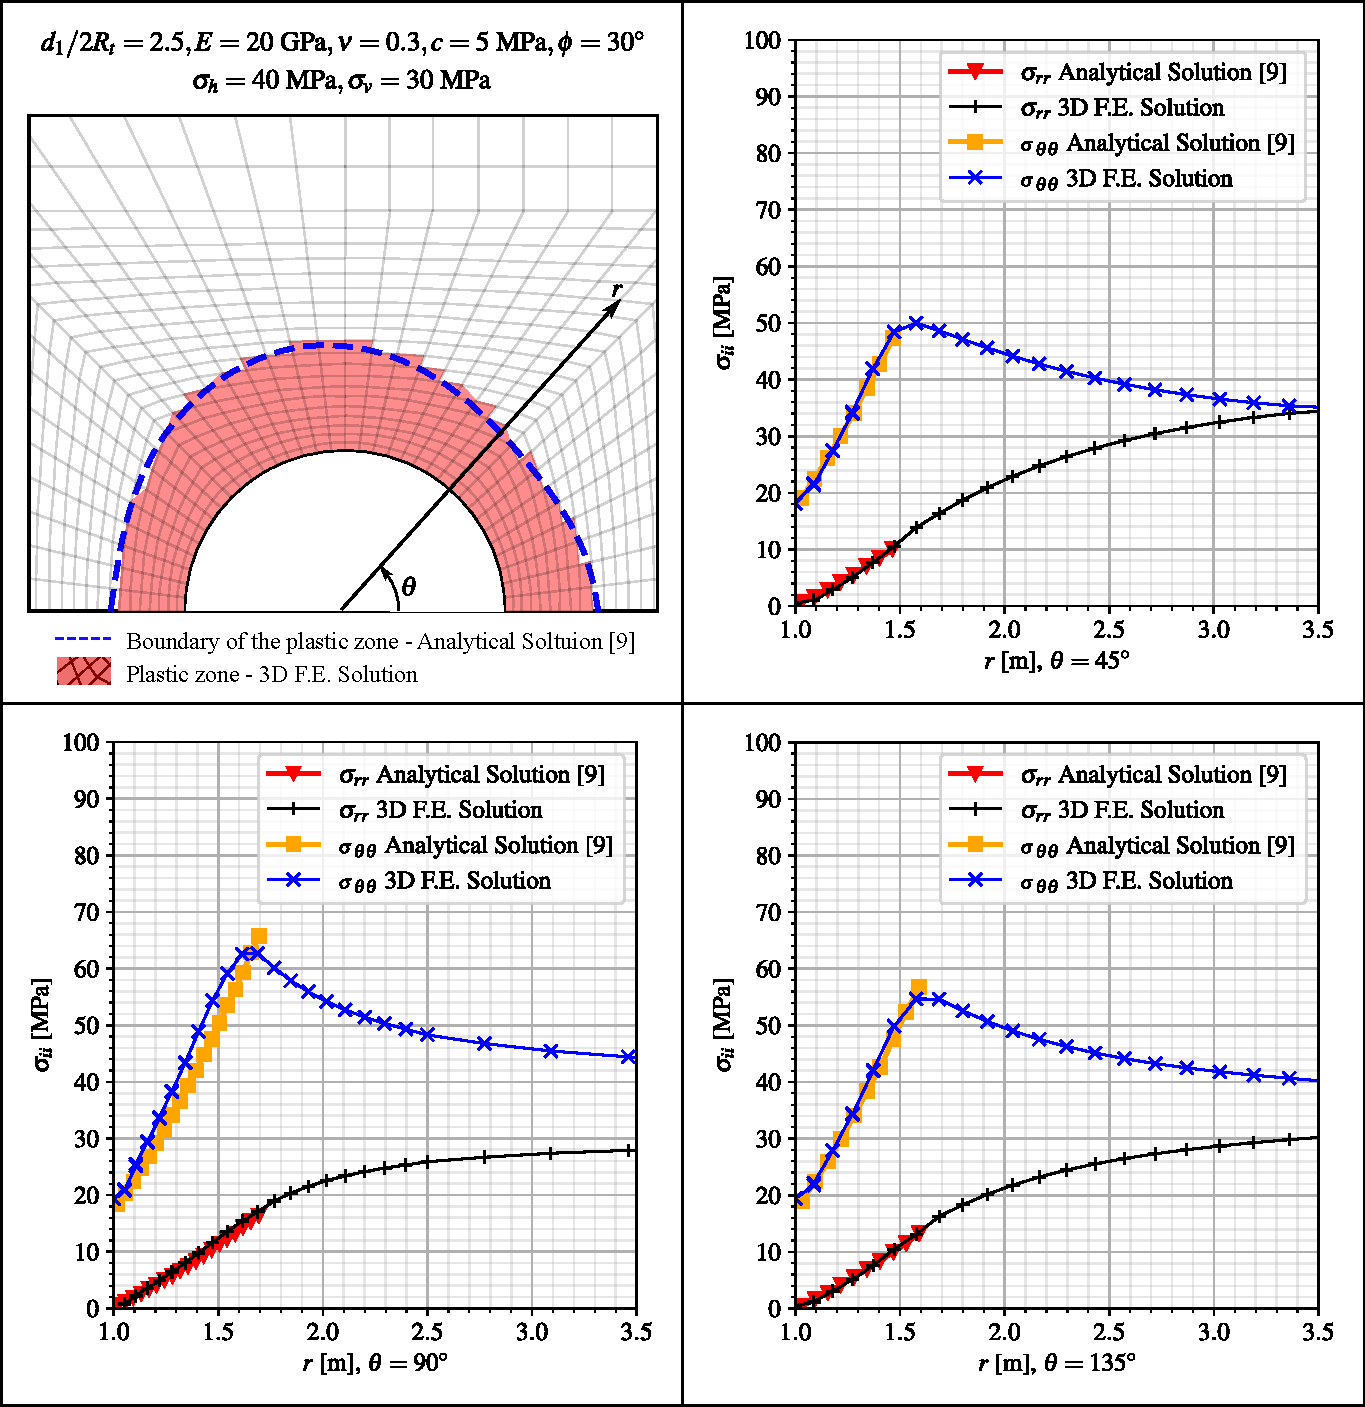
\includegraphics[scale=0.6]{MA_stresspaths.pdf}
	\caption{Distribution of radial and orthoradial stress components along different radial directions: comparison between numerical and analytical predictions.}
	\label{MA_stresspaths}
\end{figure}
\FloatBarrier

\section{Three-dimensional finite element simulations}\label{sec7}

This section provides some numerical results related to rock deformation in twin tunnels with transverse gallery obtained from the 3D computational model presented in sections ~\ref{sec3}, ~\ref{sec4} and ~\ref{section_spatial}. It is emphasized that the primary objective herein is to illustrate the capabilities of the proposed formulation to address within a 3D context the configuration of a complex tunnel structure involving nonlinear and time-dependent couplings.  Elaboration of an exhaustive parametric analysis integrating the effects of geometrical, constitutive and loading parameters is notably beyond the scope of the numerical application.

\subsection{Model data and preliminary considerations}\label{sec71}

The rock constitutive data used in the subsequent analysis refer to a deep clay from eastern Paris basin (Aisne region, France) studied in [\citenum{rousset1988}, \citenum{GIRAUD1996}, \citenum{piepi1995}, \citenum{giraud1993}]. The material properties including elastoplastic and viscoplastic parameters summarized in Table~\ref{table2} have been evaluated and calibrated from an extensive series of laboratory tests performed under undrained conditions [\citenum{rousset1988}, \citenum{piepi1995}, \citenum{giraud1993}]. The Aisne clay rocks exhibit high density (2.01 to 2.57 g/cm$^3$), a low average water content (between 3 to 11\%) and relatively low porosity (typically less than 20\%). It is therefore assumed that hydromechanical coupling can be neglected in the analysis of rock material deformation. In particular, the creep tests indicated that the long-term effects primarily stem from material viscosity, with a very low proportion induced by pore pressure redistribution. An important characteristic of the behavior such clay is that irreversible strains are observed in cyclic tests even at small values of axial strain (less than 0.3\%). The instantaneous undrained triaxial tests performed at high confining pressure values, such as those prevailing in the rock mass at approximately 450 m deep, indicated that the maximum deviatoric stress remains approximately constant, thus suggesting a Tresca-type failure criterion for the short-term component of the behavior. As for the long-term behavior, the creep tests revealed that the deviatoric stress threshold beyond which the material exhibits creep deformation is almost independent on the mean stress, suggesting that the time-dependent behavior component can be conveniently described by a Tresca-like criterion. Comparison of instantaneous and delayed behaviors reveals that short-term cohesion exceeds long-term cohesion within a ratio ranging between 1.2 and 2.  Based on these observations, the constitutive model data adopted for the elastoplastic and viscoplastic components of rock material behavior is summarized in Table~\ref{table2}.

Table~\ref{table2} also presents the constitutive parameters used for the lining used for the twin tunnels and gallery, the instantaneous relaxation modulus under uniaxial stress at 28 days being referred to as $E_{c_{28}}$. In the analyses that considers elastic behavior of the lining, the concrete elastic modulus is set equal to $E_{c_{28}}$. When viscoelastic behavior is adopted for the lining, the relaxation modulus evolves in time according to the Generalized Kelvin model described in section~\ref{sec4}, whereas the Poisson ratio is assumed to be constant within the time interval of analysis. During the tunnel construction process, loading and creep of each lining segment starts from the moment it is activated with properties at age $t_0=1$ day, whereas shrinkage effects are assumed to take part at the age of $t_s=7$ days.

\FloatBarrier
\begin{table}[h!]
	\caption{Constitutive parameters used in the numerical analysis.}
	\label{table2}
	\centering
	%\small
	\renewcommand{\arraystretch}{1.25}
	\begin{tabular}{c c c c}
		\hline
		\multicolumn{1}{c}{PARAMETERS} &
		\multicolumn{1}{c}{SYMBOL} &
		\multicolumn{1}{c}{UNIT} &
		\multicolumn{1}{c}{VALUES} \\
		\hline
		\multicolumn{4}{c}{Constitutive model of rock mass} \\
		\hline
		Young's modulus & $E$ & MPa & $1500$ \\
		Poisson's ratio & $\nu$ & - & $0.49$ \\
		Plastic cohesion & $c$ & MPa & 4$\sqrt{3}/2$ \\
		Plastic friction angle & $\phi$ & $^{\circ}$ & 0 \\
		Viscoplastic cohesion & $c_{vp}$ & MPa & 2$\sqrt{3}/2$ \\
		Viscoplastic friction angle & $\phi_{vp}$ & $^{\circ}$ & 0 \\
		Power law parameter & $n$ & - & 1 \\
		Reference parameter & $f_0$ & MPa & 1 \\
		Viscosity coefficient & $\eta$ & day & $40000$ \\
		\hline
		\multicolumn{4}{c}{Constitutive model of lining} \\
		\hline
		
		Characteristic compressive strength at age of 28 days & $f_{ck}$ & MPa & $20$ \\
		Modulus of elasticity at the age of 28 days & $E_{c_{28}}$ & MPa & $30303$ \\
		Poisson's ratio & $\nu_c$ & - & $0.2$ \\
		
		Coefficient defining instantaneous relaxation modulus [\citenum{CEB:1993}] & $s$ & - & $0.2$ \\
		Relative humidity of ambient environment & $RH$ & \% & $70$ \\
		Notional size of member - longitudinal concrete lining & $h_t$ & cm & $0.2111$ \\
		Notional size of member - gallery concrete lining & $h_{g}$ & cm & $0.2176$ \\
		Age of concrete at the beginning of shrinkage & $t_s$ & days & $7$ \\
		Shrinkage coefficient depending on cement type [\citenum{CEB:1993}] & $\beta_{sc}$ & - & $8$ \\
		Temperature & $T$ & $^\circ$C & $20$ \\
		Age of concrete at loading & $t_0$ & days & $1$ \\
		\hline
	\end{tabular}
	\normalsize
\end{table}
\FloatBarrier

The parameters defining the structure geometry as well as the excavation and lining installation process are provided in Table~\ref{table1}. All the length parameters are normalized by the tunnel radius $R_t$, which amounts to formally consider radius $R_t=1$ m in the numerical simulations. As mentioned in Table~\ref{table1}, three different values shall be considered in the simulations for the distance between twin tunnels axes, namely $d_1=4R_t$, $d_1=8R_t$, and $d_1=16R_t$. In addition, constant values of tunnel and gallery advancement rates are considered and fixed to $V_{pt} = V_{pg} = 12.5$ m/day. As regards the initial stress state prevailing prior to excavation processes, hydrostatic stress distribution with $\sigma_v=\sigma_h=9 \text{MPa}$, corresponding to geostatic conditions at depths of about of 450 m, is adopted in the subsequent simulations.

The numerical study investigates the long-term and short-term tunnel convergence profiles considering various constitutive models for the rock mass (elastic, elastoplastic, viscoplastic or elastoplastic-viscoplastic) and for the lining (elastic and viscoelastic). For the comparison purposes, the configuration of unlined tunnel as well as the configurations with or without transverse gallery will also be analyzed. To facilitate the description of the different configurations addressed below, Table~\ref{table3} provides the list of each configuration as well as associated abbreviation used to refer to in the presentation of numerical results.

\FloatBarrier
\begin{table}[h!]
	\caption{Configurations and associated abbreviations used in numerical simulations.}
	\label{table3}
	\centering
	%\small
	\renewcommand{\arraystretch}{1.25}
	\begin{tabular}{c c}
		\hline
		\multicolumn{1}{c}{DESCRIPTION} &
		\multicolumn{1}{c}{ABBREVIATION} \\
		\hline
		Elastic rock mass & E \\
		Elastoplastic rock mass & EP \\
		Elastoviscoplastic rock mass & VP \\
		Elastoplastic-Viscoplastic rock mass & EPVP \\
		No lining & NL \\
		Elastic lining & EL \\
		Viscoelastic lining & VEL \\
		Long-term & LT \\
		End of excavation process (Short-term) & ST \\
		With Gallery & WG \\
		No Gallery & NG \\			
		\hline
	\end{tabular}
	\normalsize
\end{table}
\FloatBarrier


Denoting by $u_y$ the displacement component along the vertical  $y$-axis, all the results presented in the following analyses will specifically refer the convergence profile $U_B=-u_y(B)/R_t$ that characterizes the inward movement of the tunnel roof $B(x = -d_1/2, y = R_t, z)$ as a function of the normalized algebraic longitudinal distance $z/R_t$ from the excavation face. In addition, point  $C(x=-d_1/2, y =R_t, z = -25R_t)$ has been chosen as representative of the equilibrium convergence $U_C$ far behind the tunnel face and transverse gallery. When the gallery intersects the longitudinal tunnel, the highest convergence value $U_{peak}$ highlighted in the plots of convergence curves refers to point $D(x=-d_1/2, y = R_t, z = L_1+L_2/2)$ located at the roof of longitudinal tunnel section lying at the tunnel/transverse gallery junction.

The first feature of tunnel deformation to be mentioned is related to the tunnel deformation anisotropy (or ovalization) induced by the twin tunnels proximity. A single circular tunnel excavated in a homogeneous isotropic rock mass with hydrostatic initial stress state will deform symmetrically so that the circular shape of tunnel wall will be preserved throughout the excavation process. As already pointed out in the preliminary numerical simulations presented in section~\ref{sec6}, the mutual interaction associated with twin tunnels proximity will in contrast result in anisotropic deformation of the tunnel wall, the ovalization effect being more pronounced as the distance between twin tunnels axes $d_1$ decreases. For illustrative purposes, Fig.~\ref{Ovalization effect and monitoring point} presents schematic plots of the deformed tunnel wall far behind the face together with trajectory of monitoring point B considering three different values of normalized twin tunnel spacing $d_1/R_t$. The configuration shown in this figure corresponds to elastoplastic rock mass (EP), elastic lining (EL) and transverse gallery (WG). It should be however kept in mind that due to tunnel ovalization, $U_B$ would not be therefore sufficient for characterizing the whole deformation of the tunnel wall.

\begin{figure}[h!]
	\centering
	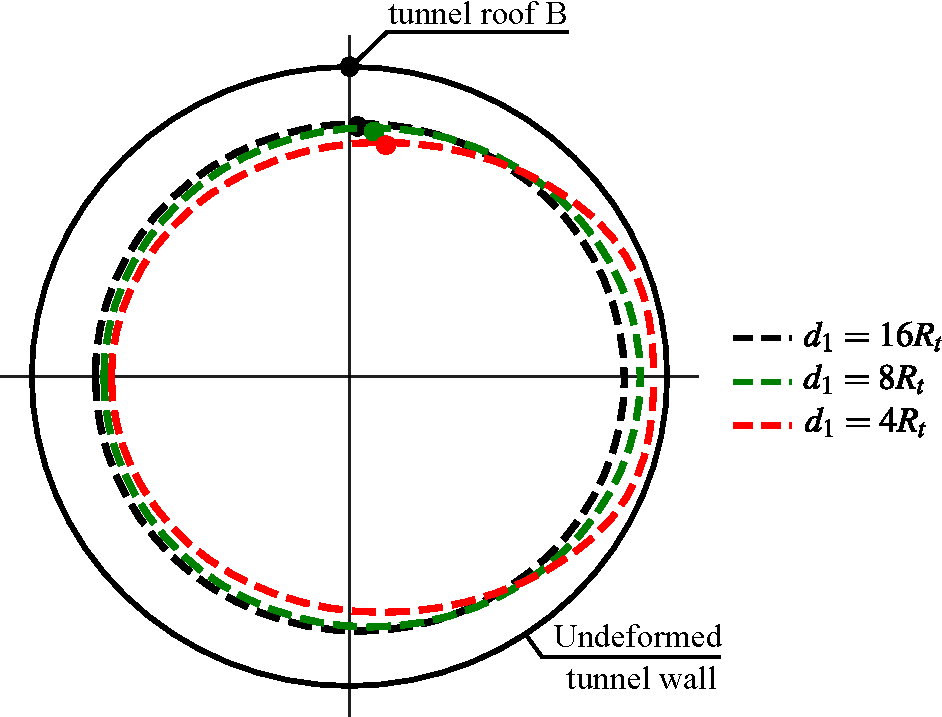
\includegraphics[scale=0.5]{Ovalization effect and monitoring point.pdf}
	\caption{Illustration of the deformation anisotropy induced by twin tunnels proximity.}
	\label{Ovalization effect and monitoring point}
\end{figure}
\FloatBarrier

The second feature of the tunnel deformation that deserves to be mentioned refer the specific deformation patterns prevailing in the region surrounding the tunnel wall. In consistence with experimental data, the plastic cohesion $c$ and viscoplastic cohesion $c_{vp}$ reported in Table~\ref{table2} comply with condition  $c > c_{vp}$. This notably implies that irreversible viscoplastic strains will be activated earlier as the tunnel excavation. Schematic representation of deformation patterns within the rock mass is illustrated in Fig.~\ref{zones}.

\begin{figure}[h!]
	\centering
	\includegraphics[scale=0.6]{zones.pdf}
	\caption{Evolution of deformation zones as the tunnel excavation proceeds.}
	\label{zones}
\end{figure}

[parei aqui]


\subsection{Short and long-term convergence profiles}\label{sec72}

Figs.~\ref{WG-ST-LT-D1-16RI}, \ref{WG-ST-LT-D1-8RI}, and \ref{WG-ST-LT-D1-4RI} show the convergence profiles in the twin tunnels with gallery (WG) considering the different constitutive models of the rock mass (E - blue, EP - yellow, VP - magenta, EPVP - red and green) and of the lining (EL and VEL). The interaction effect rising from twin tunnels proximity is investigated by considering three values $d_1=4R_t$, $d_1=8R_t$, and $d_1=16R_t$.  The solid lines refer to short-term analysis (ST) whereas the dashed lines to long-term analysis (LT).

\begin{figure}[h!]
	\centering
	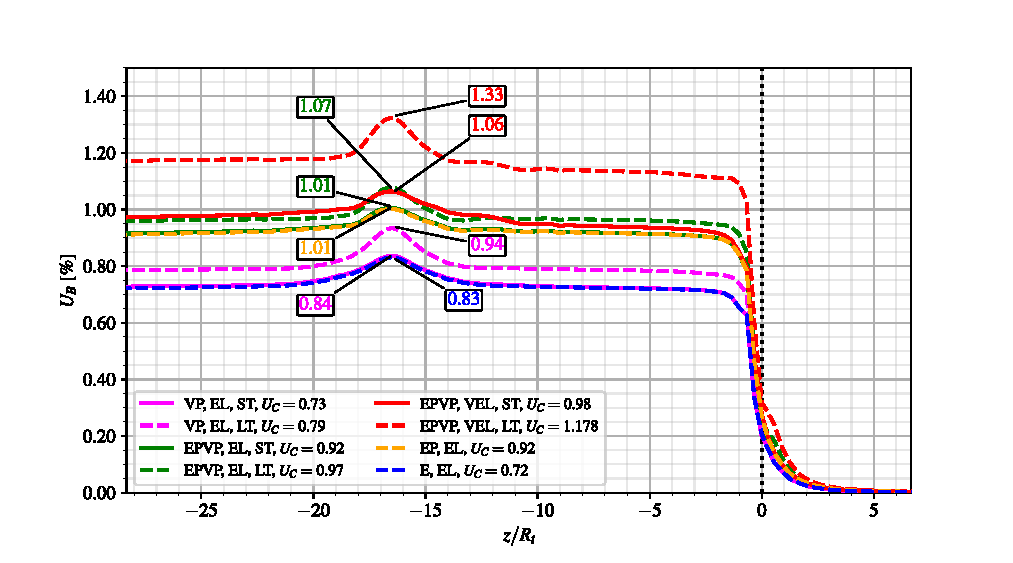
\includegraphics[scale=0.9]{Convergence Profiles - WG_ST_LT - $d_1=16R_i$_anotate.pdf}
	\caption{Convergence Profiles: short-term (ST) and long-term (LT) analyses for the configuration with gallery (WG) and distance between twin tunnels $d_1 = 16R_t$.}
	\label{WG-ST-LT-D1-16RI}
\end{figure}
\FloatBarrier
\begin{figure}[h!]
	\centering
	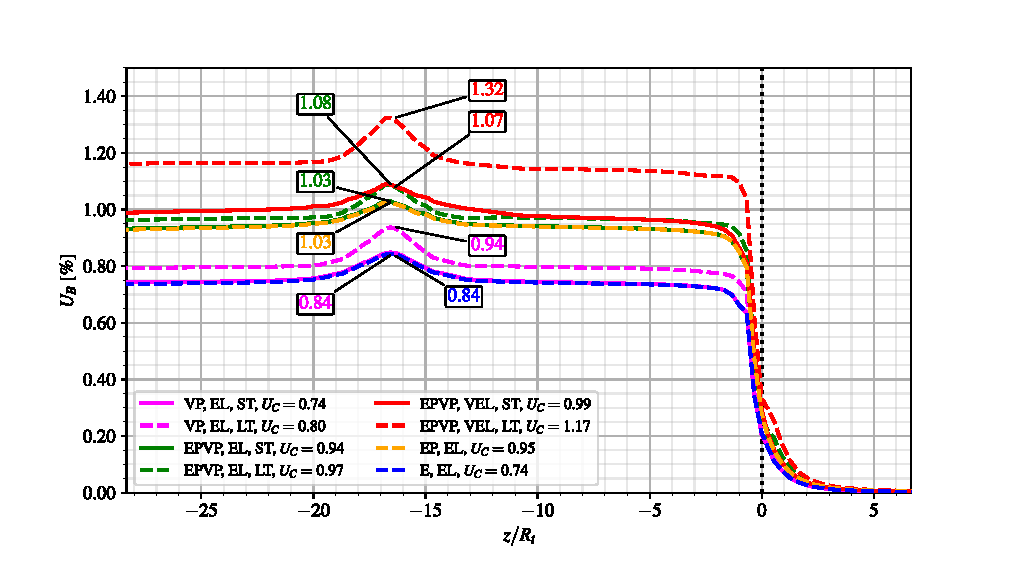
\includegraphics[scale=0.9]{Convergence Profiles - WG_ST_LT - $d_1=8R_i$_anotate.pdf}
	\caption{
		Convergence Profiles: short-term (ST) and long-term (LT) analyses for the configuration with gallery (WG) and distance between twin tunnels $d_1 = 8R_t$.}
	\label{WG-ST-LT-D1-8RI}
\end{figure}
\FloatBarrier
\begin{figure}[h!]
	\centering
	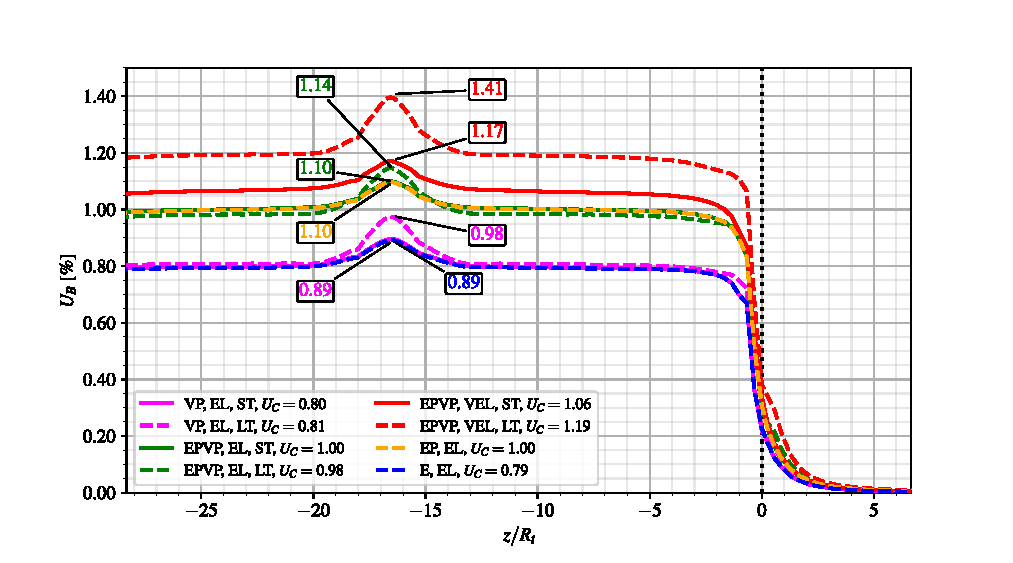
\includegraphics[scale=0.9]{Convergence Profiles - WG_ST_LT - $d_1=4R_i$_anotate.pdf}
	\caption{Convergence Profiles: short-term (ST) and long-term (LT) analyses for the configuration with gallery (WG) and distance between twin tunnels $d_1 = 4R_t$.}
	\label{WG-ST-LT-D1-4RI}
\end{figure}
\FloatBarrier

For all investigated values of twin tunnels distance $d_1$, the convergence profiles obtained in short-term (ST) analyses are very similar for both the E-EL (blue dashed line) and the VP-EL (magenta solid line) constitutive model configurations. This mainly attributed to relatively high value considered for the tunnel/gallery advancement rate and lining installation (excavation speed $V_{pt}=V_{pg}$), thus limiting the viscous effects on the tunnel deformation. The same explanation holds regarding the results derived from the short-term (ST) analyses with the EP-EL (yellow dashed line) or EPVP-EL (green solid line) constitutive model configurations. However, the viscous effects give rise to delayed tunnel deformation progressively affecting the long-term (LT) convergence (dashed green line) at the tunnel roof B. The discrepancy between short-term and long-term responses is more pronounced when a time-dependent viscoelastic lining is considered, as clearly indicated from the convergence associated with the EPVP-VEL model (solid and dashed red lines).

It is noted that the relatively high stiffness considered of the elastic lining is likely to significantly reduces the viscous component of tunnel wall deformation. This can be illustrated by analyzing the short-term and long-term convergences for VP-EL model (solid and dashed magenta line). In this configuration, the twin tunnels proximity induces a substantial increase in the short-term (ST) prediction of $U_C$ when comparing $d_1=8R_t$ and $d_1=4R_t$, whereas the long-term (LT) convergence hardly changes mainly due to the restriction imposed by the stiff lining.

Referring to the configuration analyzed in Figs.~\ref{WG-ST-LT-D1-16RI}, \ref{WG-ST-LT-D1-8RI}, and \ref{WG-ST-LT-D1-4RI}, the ovalization effect may be illustrated by visualizing in Fig.~\ref{ovalization}~the anisotropic deformation of  a tunnel cross-section located far behind the face  in the particular case of twin tunnel distance $d_1=4R_t$. In this figure, the configuration of a single circular tunnel ($d_1 \rightarrow \infty$) is also shown as a reference case. 

\begin{figure}[h!]
	\centering
	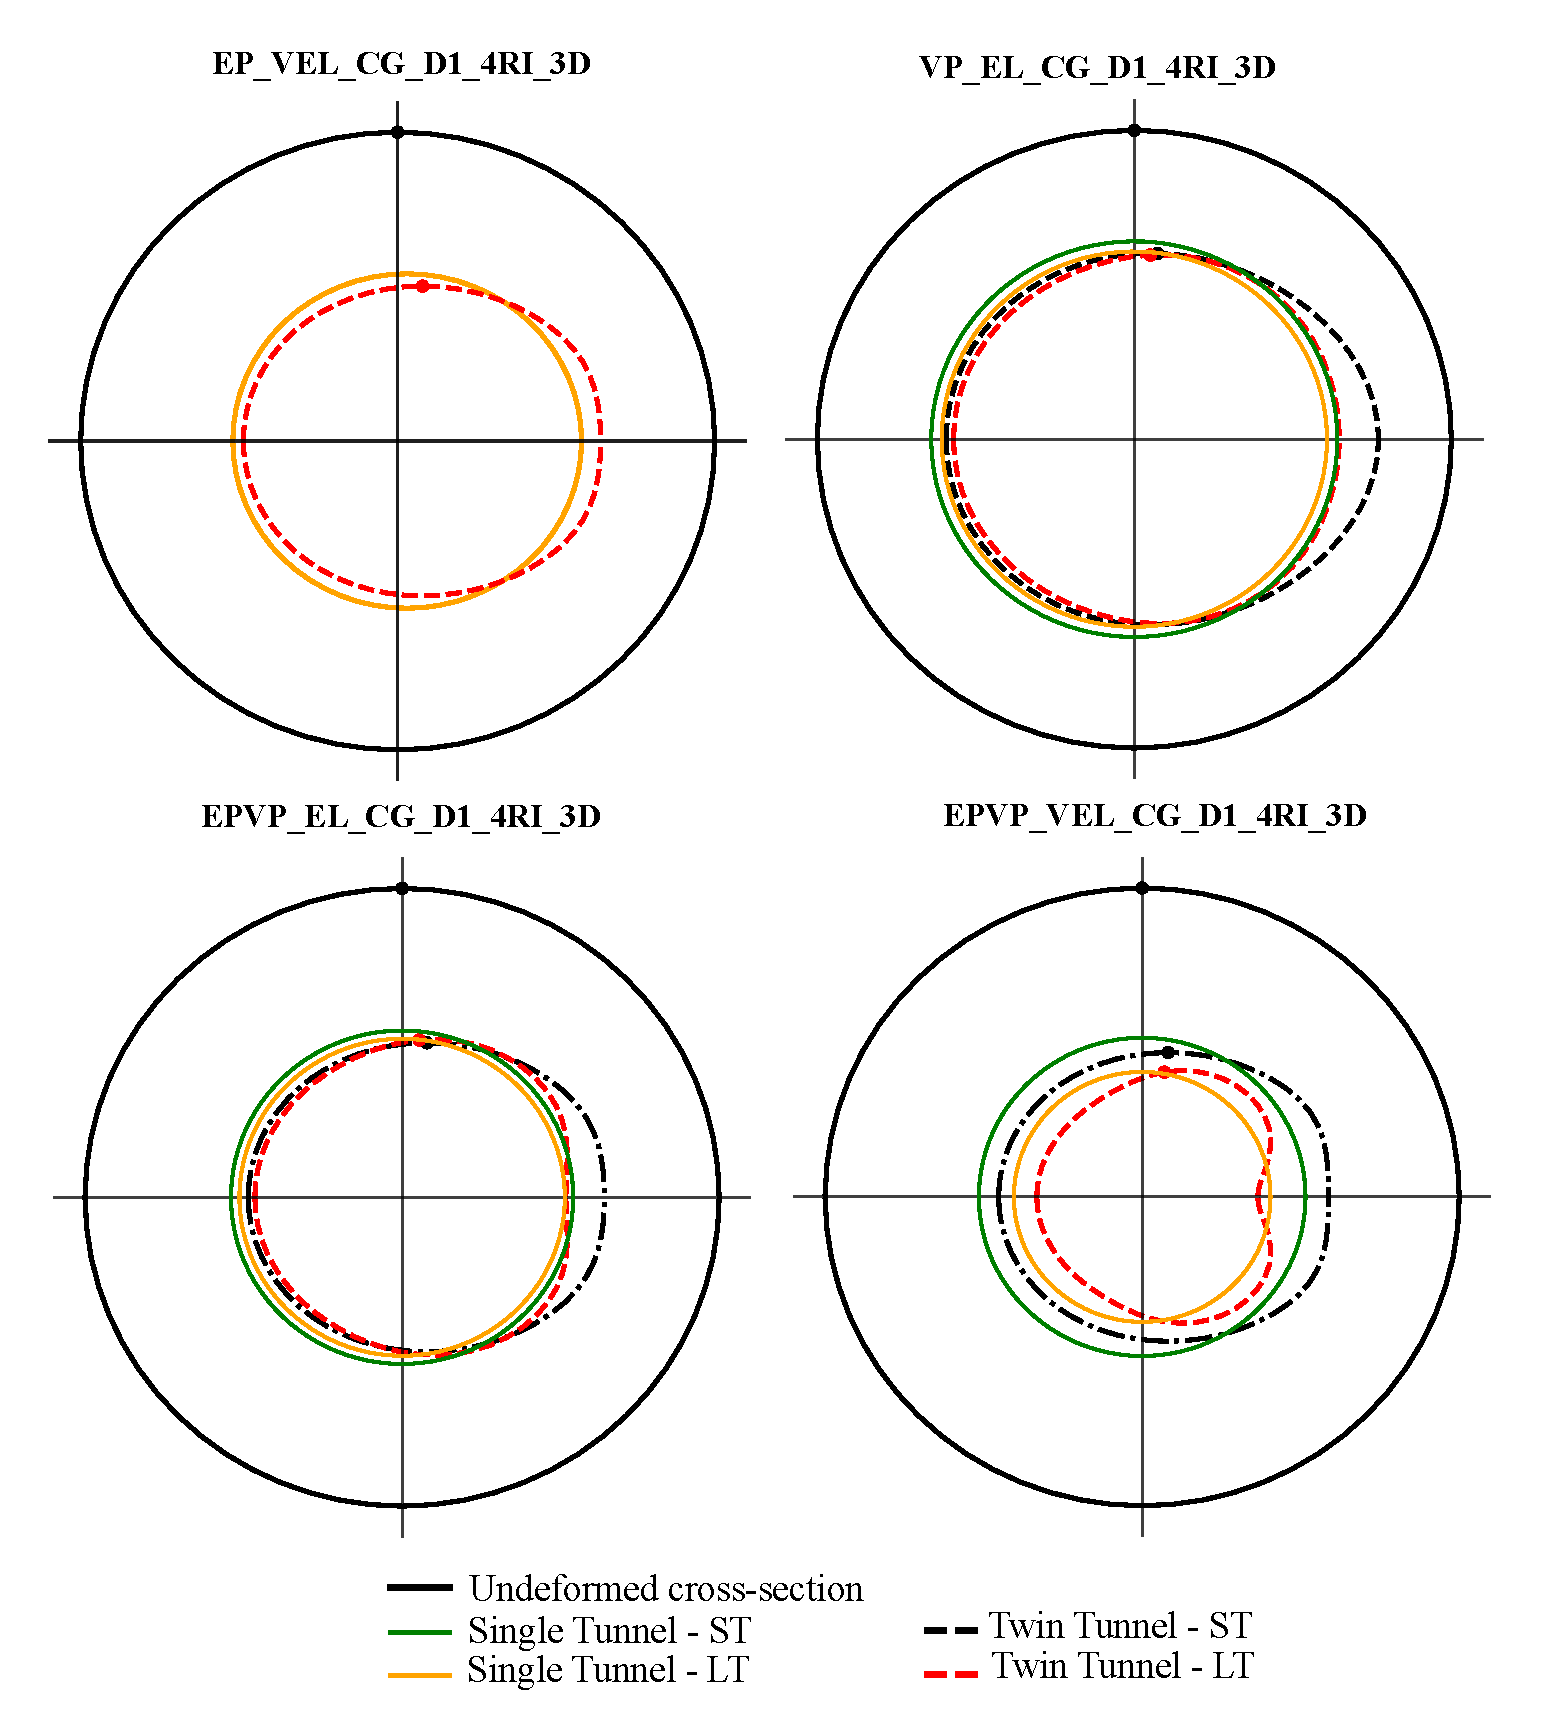
\includegraphics[scale=0.4]{ovalization.pdf}
	\caption{Illustration of deformation anisotropy induced: configuration with gallery (WG) and distance between twin tunnels $d_1 = 4R_t$.}
	\label{ovalization}
\end{figure}
\FloatBarrier

In that respect, Fig.~\ref{UB-UAUB-D1_4RT} provides further illustration of the ovalization effect by plotting the anisotropy ratio $U_B/U_A = u_y(B)/u_x(A)$ between the vertical displacement $u_y$ at the roof B and the horizontal displacement $u_x$ at the side wall $A(x=R_t - d_1/2,y=0,z)$. The resulted presented in this figure correspond to twin tunnels without transverse gallery (NG) and distance $d_1=4R_t$. The results suggest a more pronounced ovalization effect short-term tunnel deformation (solid lines).

\begin{figure}[h!]
	\centering
	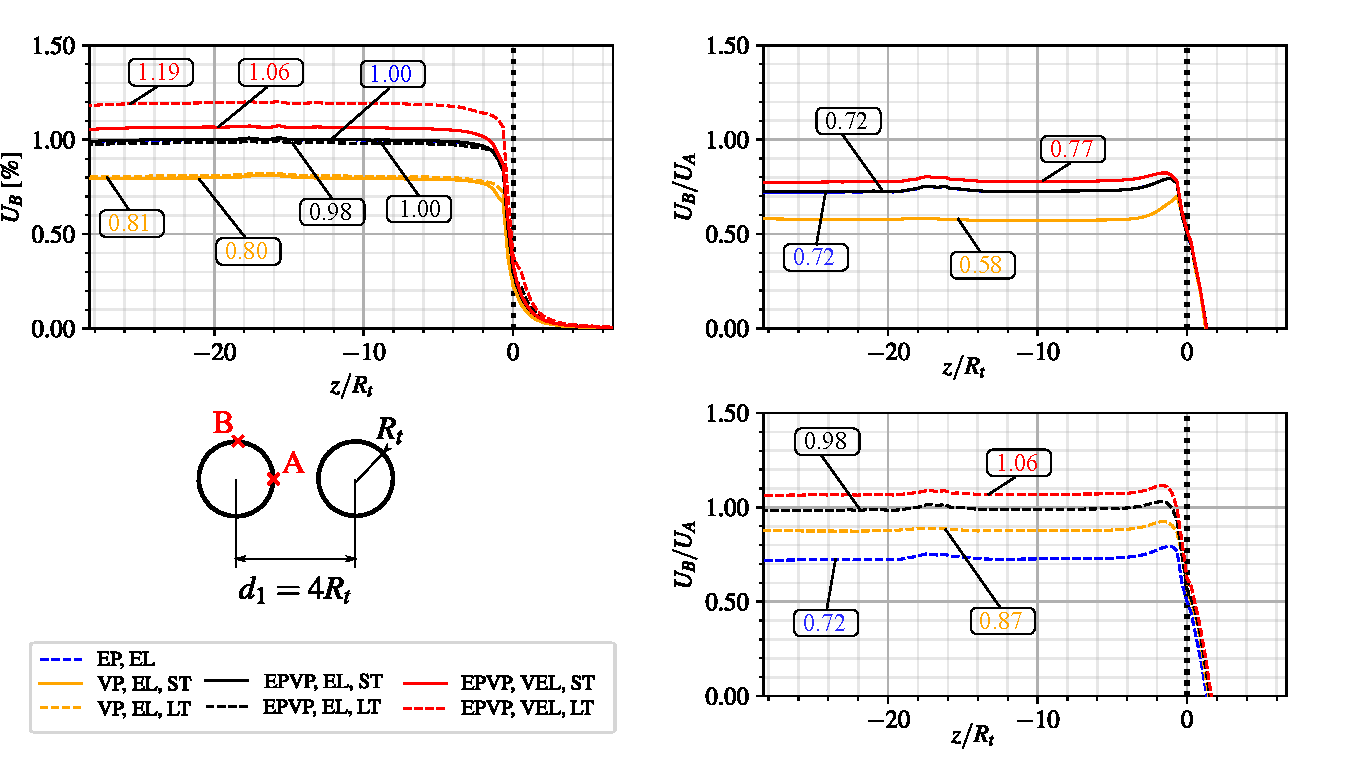
\includegraphics[scale=0.65]{Convergence Profiles - UB - UAUB - $d_1=4R_t - ST_Lt$.pdf}
	\caption{Deformation anisotropy induced by twin tunnels proximity for the configuration without gallery (NG) and distance between twin tunnels $d_1=4R_t$: (a) convergence profile at the tunnel roof B, (b) anisotropy ratio obtained in short-term analysis, (c) anisotropy ratio obtained in long-term analysis.}
	\label{UB-UAUB-D1_4RT}
\end{figure}
\FloatBarrier

\subsection{Additional numerical analysis: impact of creep deformation}\label{sec73}

This section provides further numerical results obtained from long-term and short-term analyses, with particular emphasis on the effect of time-dependent behavior of the rock material and lining constituent materials. Fig.~\ref{VP-EL-EPVP-VEL-WG-LT} displays the long-term convergence profiles for $d_1=16R_t$, $8R_t$ and $4R_t$ (yellow, green and red lines, respectively) considering viscous constitutive models: viscoplastic rock mass with elastic lining (VP-EL - solid lines), elastoplastic-viscoplastic rock mass with elastic lining (EPVP-EL - dashed line) and viscoelastic lining (EPVP-VEL - dotted lines). To emphasize the interaction rising from twin tunnels proximity and transverse gallery, the results obtained in the reference configuration of a single tunnel (black lines) are also shown. Close values of the peak convergence  $U_{peak}$ are obtained at the tunnel roof for the EPVP-VEL model with $d_1=16R_t$ (yellow dotted line) and with $d_1=8R_t$ (green dotted line). This result may be explained by the fact the overall interaction effect on tunnel convergence results from the competing effects of twin tunnel proximity (defined by $d_1$) and the time necessary for complete gallery excavation and its intersection with longitudinal tunnel (also defined by length by $d_1$). The results indicated that these competing phenomena lead to equivalent overall effect in the cases of $d_1=8R_t$ and $d_1=16R_t$. In the case of $d_1=4R_t$ (red dotted line), the effect of twin tunnel proximity appears to be predominant, which lead to higher value of the peak convergence  $U_{peak}$.

Referring to EPVP-VEL and EPVP-EL models (dotted lines and dashed lines), it can be seen from the results of Fig.~\ref{VP-EL-EPVP-VEL-WG-LT} that higher convergence values are associated with time-dependent behavior of the lining. Unlike the stiff elastic lining, the aging viscoelastic lining induces evolving tunnel convergence along the excavation process.

\begin{figure}[h!]
	\centering
	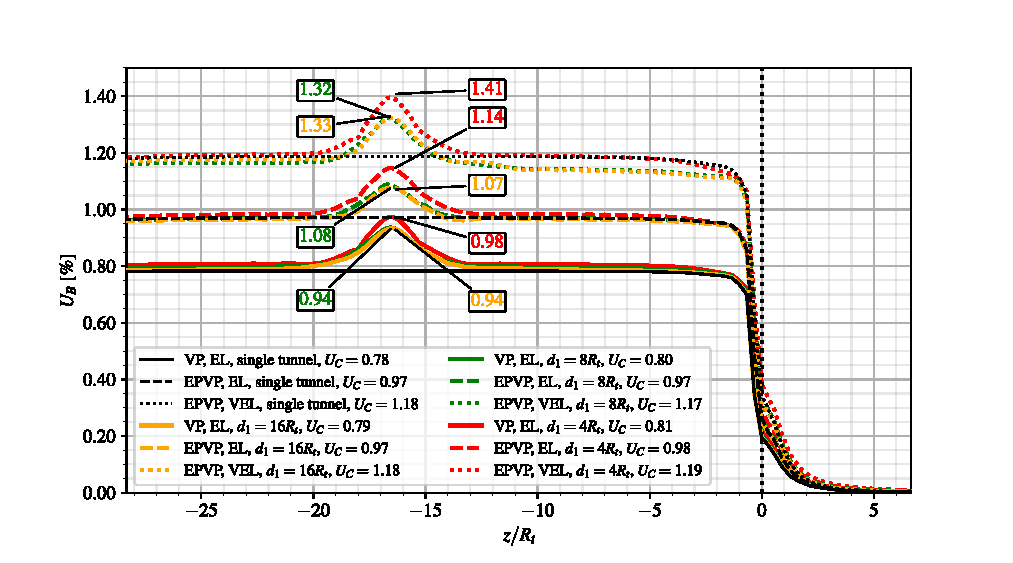
\includegraphics[scale=0.9]{Convergence Profiles - VP_EPVP_EL_VEL_WG_LT_anotate.pdf}
	\caption{Long-term convergence profiles for the configuration of twin tunnels with transverse gallery (WG): effect of rock mass and lining creep deformation.}
	\label{VP-EL-EPVP-VEL-WG-LT}
\end{figure}
\FloatBarrier

The impact of creep deformation on the tunnel convergence can alternatively be illustrated based on the comparison of the numerical predictions obtained in the cases of instantaneous behavior (elastoplastic, elastic) and time-dependent behavior (viscoplastic, viscoelastic) for the constituent materials. Fig.~\ref{EP-EL-EPVP-VEL-WG-ST-LT} depicts the convergence profiles obtained for $d_1=16R_t$, $8R_t$ and $4R_t$ (yellow, green and red lines, respectively) considering the configurations of elastoplastic rock mass with elastic lining (EP-EL - solid lines), elastoplastic-viscoplastic rock mass with viscoelastic lining in short-term analysis (EPVP-VEL-ST - dotted lines) and elastoplastic-viscoplastic rock mass with viscoelastic lining in long-term analysis (EPVP-VEL-LT - dashed lines). The case of single circular tunnel ($d_1  \rightarrow \infty$) is also analyzed as reference configuration (black lines).

\begin{figure}[h!]
	\centering
	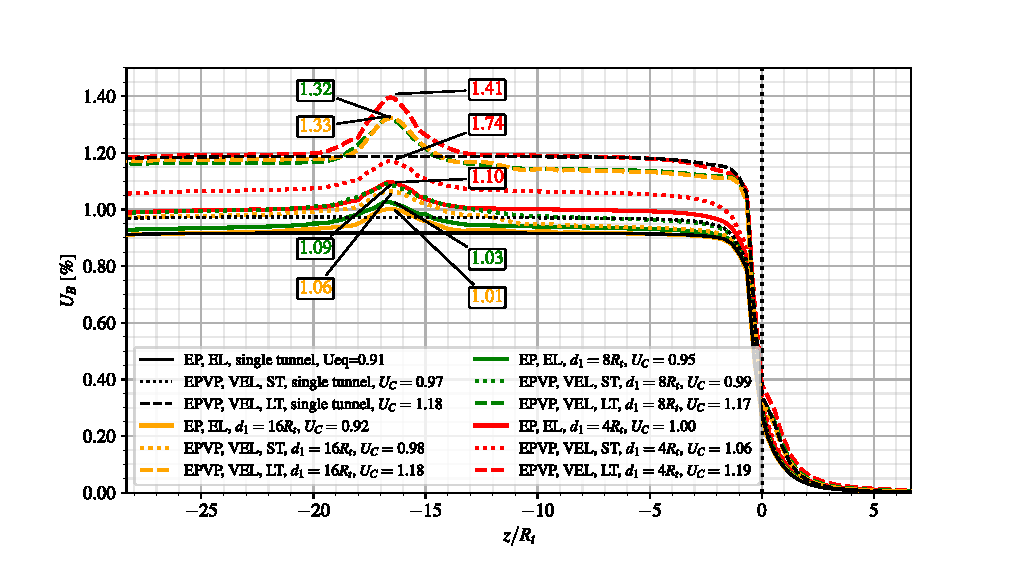
\includegraphics[scale=0.9]{Convergence Profiles - EP_EL_EPVP_VEL_WG_ST_LT_anotate.pdf}
	\caption{Short-term and long-term convergence profiles obtained for the configuration of twin tunnels with transverse gallery (WG): instantaneous versus delayed behaviors of the rock and lining constituent material.}
	\label{EP-EL-EPVP-VEL-WG-ST-LT}
\end{figure}
\FloatBarrier

Once again, the result predictions shown in this figure emphasize the significative impact of the viscoelastic lining behavior on the short-term convergence profile of the tunnels. At short-term (ST), the elastoplastic-viscoplastic rock mass with viscoelastic lining (EPVP-VEL - dotted lines) leads to higher convergences when compared to the elastoplastic rock mass with elastic lining (EP-EL - solid lines). This is mainly attributed to the fact the early age viscoelastic lining (VEL) exhibits lower relaxation modulus than the stiffness $E_{c_{28}}$ considered for elastic lining (EL), thus resulting in higher tunnel deformation. Regarding the long-term analysis (LT), even though the viscoelastic lining (VEL) (dashed lines) exhibit increasing relaxation modulus due to aging phenomenon, the creep deformation of both the rock and lining constituents result in significantly higher convergences at the tunnel roof when compared to obtained for elastoplastic rock with elastic lining (EP-EL - solid lines). A noticeable increase in the magnitude of $U_{peak}$, induced by the interaction with transverse gallery, is also observed from the short-term response (dotted lines) to the long-term response (dashed lines), highlighting once again the influence of the delayed behavior of the rock and the lining.

\subsection{Effect of the lining stiffness on the tunnel convergence}\label{}

In tunnel deformation analyses, the behavior of the concrete lining is classically characterized by the elastic stiffness parameter, which relates the normal stress exerted by the surrounding the rock mass and the normalized lining normal displacement (convergence).   The elastic stiffness parameter is computed from the elastic properties of concrete material and the lining thickness (normalized by the tunnel radius) [\citenum{Panet1995}, \citenum{brown1980}]. This concept is extended herein to case of viscoelastic lining by in traducing the instantaneous stiffness modulus at 28 days $K_{c_{28}}$ as:

\begin{equation} \label{eq:Kc}
	K_{c_{28}} = \frac{E_{c_{28}}}{1+\nu_c}\frac{1-(1-e_t/R_t)^2}{(1-2\nu_c)+(1-e_t/R_t)^2}
\end{equation}

In the above analyses of sections~\ref{sec71}, \ref{sec72} and \ref{sec73} the lining thickness were fixed to $e_t=e_g=0.1R_t$, corresponding to lining stiffness  $K_{c_{28}}=3400$ MPa. As far as the tunnel deformation is concerned, the latter value characterizes a rather stiff lining, which might be a predominating factor for the control of tunnel convergence.

To assess the effect of the lining stiffness on the convergence profile, a smaller value $e_t=e_g=0.03R_t$, corresponding to lining stiffness modulus $K_{c_{28}}=970$ MPa, will be in the numerical simulations. Referring to the particular case of a rock mass exhibiting elastoplastic behavior (EP), that is only instantaneous behavior, Fig.~\ref{EP_d1_16Ri} and Fig.~\ref{EP_d1_4Ri} display the convergence profiles at tunnel roof predicted respectively for $d_1=16R_t$ and $d_1=4R_t$.  Three configurations for the support lining are considered: unlined structure (NL - dashed lines), elastic lining with lower stiffness $K_{c_{28}}=970$ - dotted lines), and elastic lining with higher stiffness $K_{c_{28}}=3400$ - solid lines). In addition, the numerical simulations include the cases with transverse gallery (WG - blue lines) and without gallery (NG - yellow lines). The reference configuration of a single tunnel is also studied (black lines). 

\begin{figure}[h!]
	\centering
	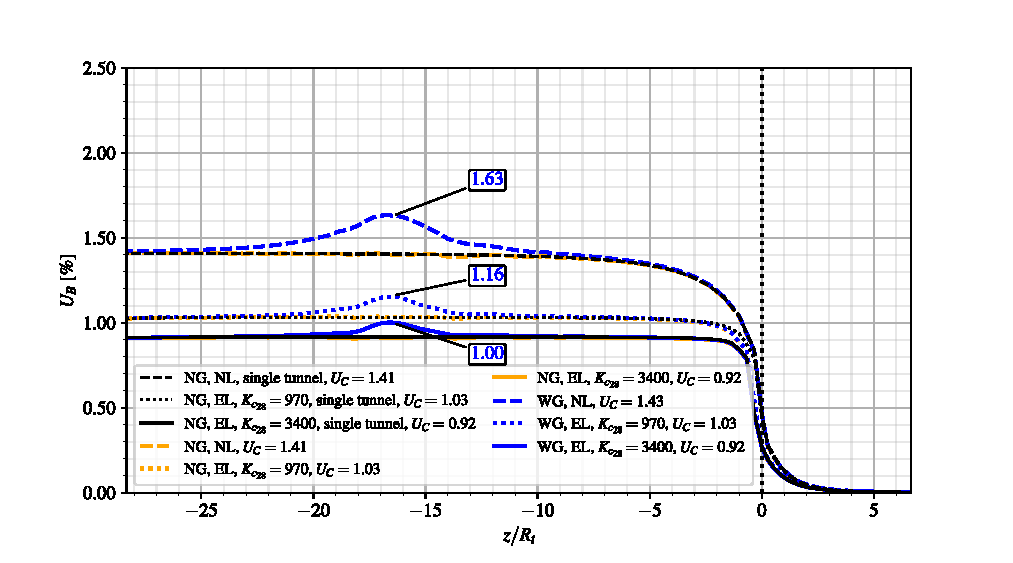
\includegraphics[scale=0.9]{Convergence Profiles - EP_d1_16Ri_anotate.pdf}
	\caption{Effect of lining stiffness on the convergence profiles for the configuration of twin tunnels with and without transverse gallery and distance between twin tunnels $d_1=16R_t$ - elastoplastic rock mass, without and with elastic lining.}
	\label{EP_d1_16Ri}
\end{figure}
\FloatBarrier
\begin{figure}[h!]
	\centering
	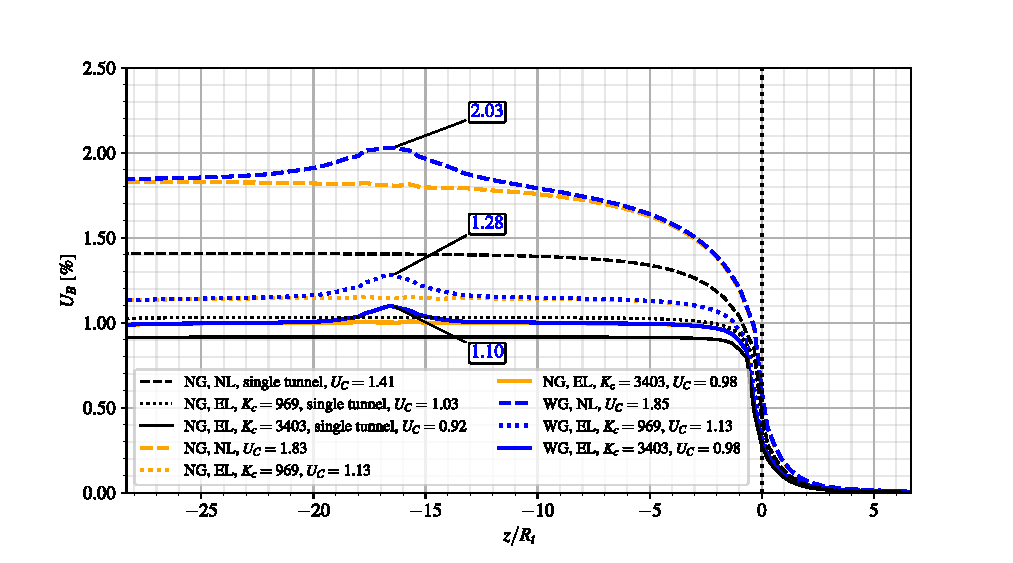
\includegraphics[scale=0.9]{Convergence Profiles - EP_d1_4Ri_anotate.pdf}
	\caption{Effect of lining stiffness on the convergence profiles for the configuration of twin tunnels with and without transverse gallery and distance between twin tunnels $d_1=4R_t$ - elastoplastic rock mass, without and with elastic lining.}
	\label{EP_d1_4Ri}
\end{figure}
\FloatBarrier

As observed in the simulations of preceding sections, the equilibrium convergence $U_C$ far behind the tunnel face is almost unaffected by the presence of transverse gallery. 

Regarding first the effect of lining stiffness on the convergence of single tunnel, the stiffer lining (black solid line) leads to a stabilized convergence reduction of approximately 35\% with respect to unlined structure (black dashed line), whereas this reduction is only 12\% for the moderate stiffness lining (black dotted line).

For twin tunnels with spacing $d_1=16R_t$, the predictions of stabilized convergence $U_C$ (blue and yellow lines) provided in Fig.~\ref{EP_d1_16Ri} are close for each lining configuration to those obtained for a single tunnel (black lines). In contrast, the interaction between the twin tunnels reveals significative when the spacing reduces to $d_1=4R_t$. In that case, the combined impact of lining support and twin tunnels proximity can be assessed by comparing in Fig.~\ref{EP_d1_4Ri} the values of convergence $U_C$ predicted for $d_1=4R_t$ (yellow and blue solid lines) and $d_1 \rightarrow \infty$ (single tunnel - black lines). Compared to the convergence of single tunnel, the increase in convergence induced by twin tunnels proximity reaches values of 30\% for unlined structure, 10\% for the moderate stiffness lining  and 6.5\% for the higher stiffness stiff. 


Analyzing the effect of lining stiffness on the disturbed region associated along the convergence profile with the presence of transverse gallery, it is first observed that the increase in stiffness reduces in all studied configurations the extent of the disturbed region, whereas the twin tunnels spacing has little impact. For the configuration of spacing $d_1=16R_t$, where the interaction due to twin tunnels proximity is expected to be minor,   the ratio $(U_{peak}-U_C)/(U_C)$ defining the relative variation between peak value and stabilized tunnel roof convergence is about 14\%, 12.5\% and 8.7\% according to the lining stiffness value: $K_{c_{28}}=0$ (unlined), $K_{c_{28}}=970$ MPa and $K_{c_{28}}=3400$ MPa. The values of this ratio are altered to about 9.7\%, 13\% and 12\% for the configuration with spacing $d_1=4R_t$ in which both effects of lining stiffness and tunnels proximity are simultaneously acting.

In line with the previous analysis investigating the impact of instantaneous stiffness modulus $K_{c_{28}}$ of the lining, Fig.~\ref{EPVP_VEL_d1_16Ri} and Fig.~\ref{EPVP_VEL_d1_4Ri} present the long-term convergence results in the configurations of elastoplastic-viscoplastic rock mass (EPVP) and  viscoelastic lining (VEL) with gallery (WG - blue lines) and without gallery (NG - yellow lines), considering  twin tunnels spacing $d_1=16R_t$ and $4R_t$, respectively. The results obtained for the reference single tunnel configuration are also provided (black lines).

Similar to the previous analysis involving constituent materials that exhibit only instantaneous behaviors, the results Fig.~\ref{EPVP_VEL_d1_16Ri} indicate that the predictions of stabilized convergence $U_C$ in the case of twin tunnels with spacing $d_1=16R_t$ are very close to obtained for single tunnel.

\begin{figure}[h!]
	\centering
	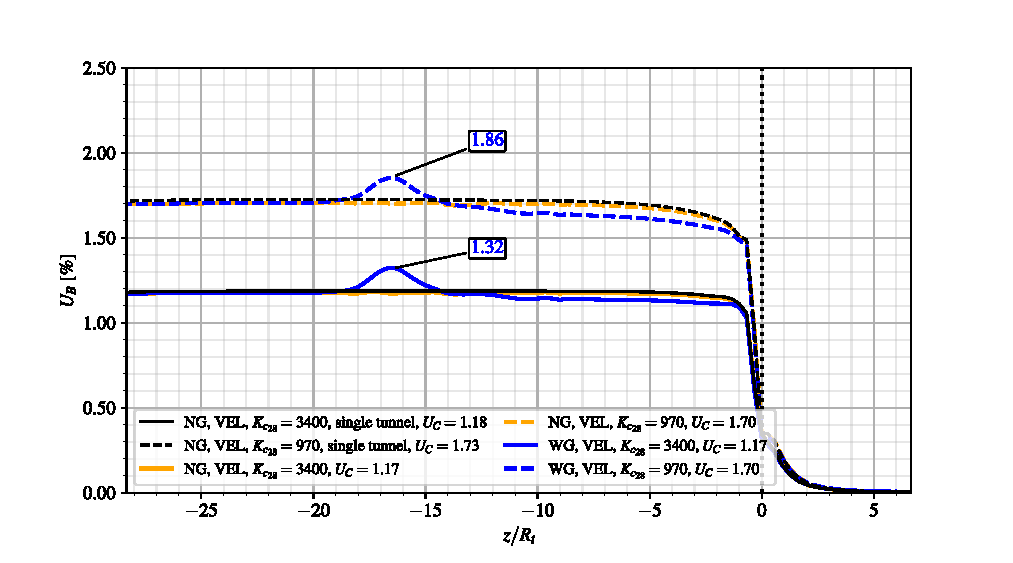
\includegraphics[scale=0.9]{Convergence Profiles - EPVP_VEL_d1_16Ri_anotate.pdf}
	\caption{Effect of instantaneous lining stiffness on the long-term convergence profiles for the configuration of twin tunnels with and without transverse gallery and distance between twin tunnels $d_1=16R_t$ - elastoplastic-viscoplastic rock mass with viscoelastic lining.}
	\label{EPVP_VEL_d1_16Ri}
\end{figure}
\FloatBarrier
\begin{figure}[h!]
	\centering
	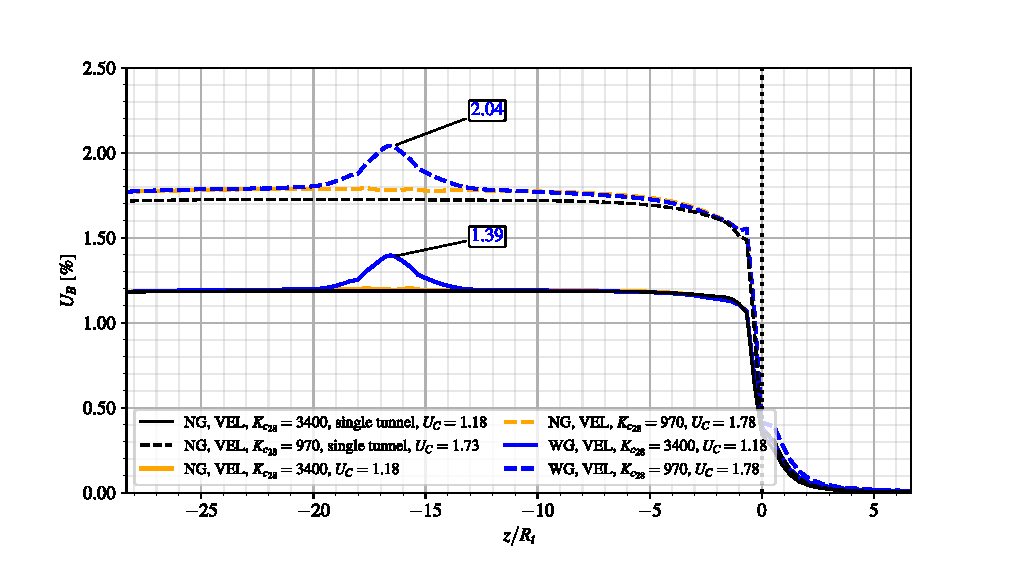
\includegraphics[scale=0.9]{Convergence Profiles - EPVP_VEL_d1_4Ri_anotate.pdf}
	\caption{Effect of instantaneous lining stiffness on the long-term convergence profiles for the configuration of twin tunnels with and without transverse gallery and distance between twin tunnels $d_1=4R_t$ - elastoplastic-viscoplastic rock mass with viscoelastic lining.}
	\label{EPVP_VEL_d1_4Ri}
\end{figure}
\FloatBarrier

Even in the specific case of $d_1=4R_t$ where a strong twin tunnels interaction would be expected, the role of lining with higher stiffness on stabilized convergence (blue and yellow solid lines in Fig.~\ref{EPVP_VEL_d1_4Ri}) is predominating with values close to obtained for single tunnel (black solid line in Fig.~\ref{EPVP_VEL_d1_4Ri}), thus masking such interaction effect. For lower lining stiffness, the numerical results (blue and yellow dashed lines) indicate a small increase in the value of  $U_C$  when compared to the single tunnel (black dashed line).

As regards the impact on the peak convergence $U_{peak}$ and extent of the gallery influence zone (disturbed portion of convergence profile), the results show that for each value of twin tunnels spacing $d_1$, the latter extent is slightly affected by the instantaneous lining stiffness modulus. In contrast the ratio $(U_{peak}-U_C)/U_C$ is significantly affected by the values of $d_1$ and  $K_{c_{28}}$. For the configuration with $d_1=4R_t$, it respectively takes the values $(U_{peak}-U_C)/U_C=$14.5\% and 18\% lower and higher lining stiffness, whereas it respectively takes the values 9.5\% and 13\% for the configuration with $d_1=16R_t$. 

\begin{figure}[h!]
	\centering
	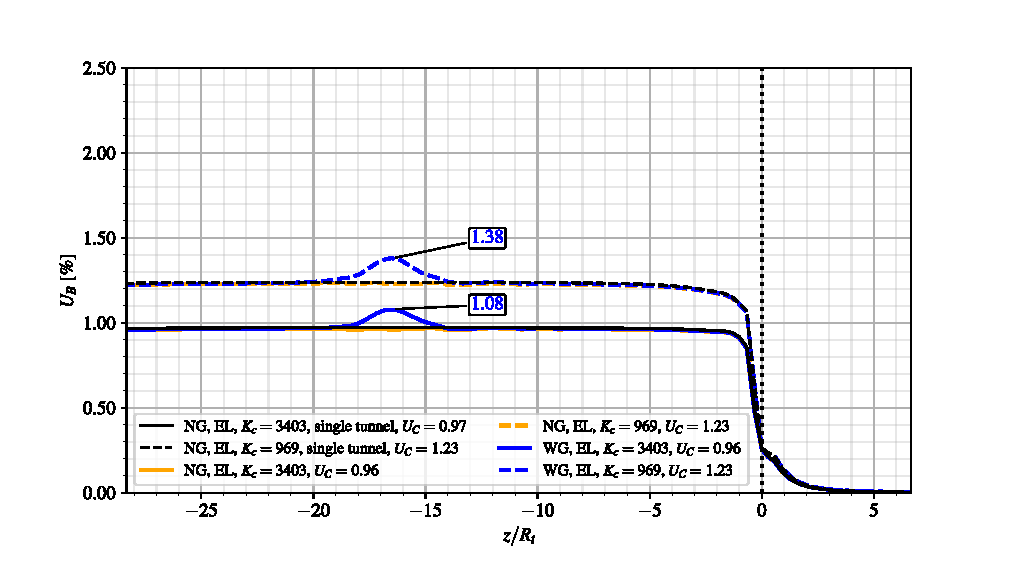
\includegraphics[scale=0.9]{Convergence Profiles - EPVP_EL_VEL_d1_16Ri_anotate.pdf}
	\caption{Effect of lining stiffness on the long-term convergence profiles for the configuration of twin tunnels with and without transverse gallery and distance between twin tunnels $d_1=16R_t$ - elastoplastic-viscoplastic rock mass with elastic lining.}
	\label{EPVP_EL_VEL_d1_16Ri}
\end{figure}
\FloatBarrier
\begin{figure}[h!]
	\centering
	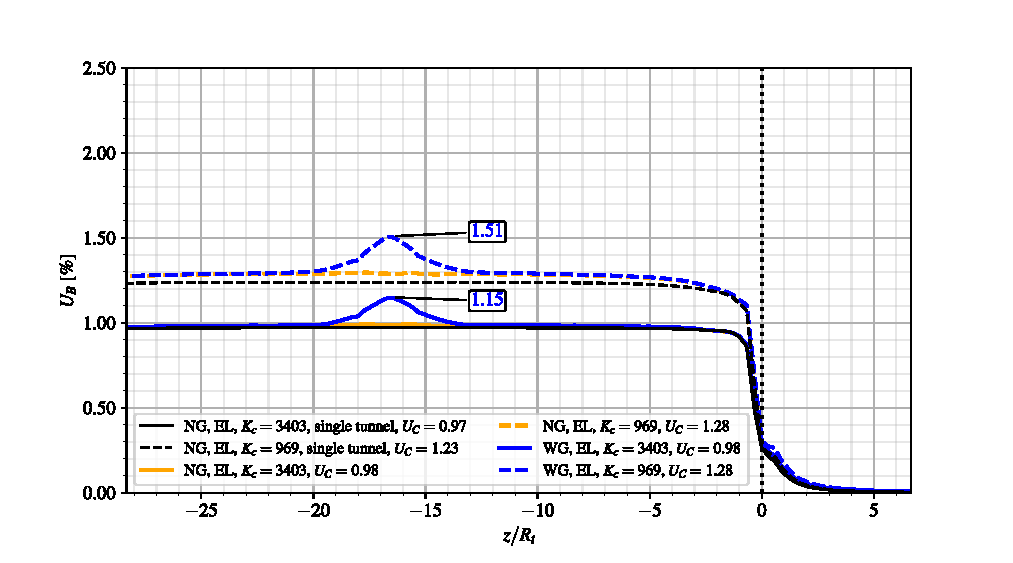
\includegraphics[scale=0.9]{Convergence Profiles - EPVP_EL_VEL_d1_4Ri_anotate.pdf}
	\caption{Effect of lining stiffness on the long-term convergence profiles for the configuration of twin tunnels with and without transverse gallery and distance between twin tunnels $d_1=4R_t$ - elastoplastic-viscoplastic rock mass with elastic lining.}
	\label{EPVP_EL_VEL_d1_4Ri}
\end{figure}
\FloatBarrier

Overall, the same observations formulated in the previous analyses regarding the effect of twin tunnel spacing on stabilized convergence still hold: with respect to single tunnel configuration, $U_C$ is almost unaffected by the lining stiffness for $U_C$  and slightly increased (up to 4\%) for $d_1=4R_t$.

With the elastic lining, the increase in stiffness from $K_{c_{28}}=970$ MPa to $K_{c_{28}}=3400$ MPa leads to a reduction in stabilized convergence $U_C$ by 28\% for twin tunnels spacing  $d_1=16R_t$ and by 16\% for $d_1=4R_t$, emphasizing once again the strong mechanical interaction between the different components of the tunnel structure.

The peak value of tunnel roof convergence $U_{peak}$ that reflects the coupling associated with intersecting transverse gallery is almost unaffected by the lining stiffness, at least for considered data parameters. In that respect, the value of ratio $(U_{peak}-U_C)/U_C$ computed in the configuration $d_1=16R_t$ (resp. $d_1=4R_t$) is  approximately 12\% (resp. and 18\%) for both values of lining stiffness, which corroborates the predominating effect of tunnels proximity on peak convergence $U_{peak}$. 

\section{Conclusions}\label{}

The paper presented a constitutive and computational model for addressing the deformation processes and mechanical interactions in deep twin tunnels with connecting transverse gallery. From the constitutive viewpoint, the irreversible component of rock deformation is modeled within the context of coupled plasticity–viscoplasticity. The latter framework is particularly relevant to describe both instantaneous and delayed deformation in deep clayey rocks. Emphasis has been devoted to the formulation of aging time-dependent constitutive properties of the lining constituent material with account for shrinkage and creep deformation, which are fundamental components of early age and long-term behavior of shotcrete support. At the structure level, the computational modeling integrates the nonlinear and time-dependent constitutive features with implementation of the activation-deactivation technique for simulating the processes of excavation and lining installation. The elaborated model is specifically devised for dealing with three-dimensional finite element analysis of deformation in twin tunnels/transverse gallery system, notably in the perspective of providing technical guidance for safe design of tunnel-gallery junction.

Conceived to provide preliminary insight into the impact of some relevant parameters defining the interaction problem, the numerical simulations undertaken in section~\ref{sec7} notably emphasized that:

\begin{enumerate}[(a)]
	
	\item The deformation anisotropy of the tunnel wall induced by twin tunnel proximity can be significant at both short-term and long-term deformation even when a stiff lining is used. This feature should therefore be integrated in the support design stage.
	
	\item The disturbed region with localized extent near the tunnel-gallery junction, reflecting the strong interaction between these two components of the structure, exhibits peak convergence values that can exceed by a large amount that the convergence far behind the facing. In that respect, the study presents the potential to formulated technical guidance for the design of twin tunnels with transverse gallery.
	
	\item In addition to the effects of coupled plastic-viscoplastic constitutive properties of the rock material, the aging time-dependent behavior considered for the lining concrete/shotcrete has a considerable impact on the short-term and long-term convergence profiles of the tunnel. In particular, the aging viscoelastic lining reveals more efficient in controlling the long-term tunnel convergence than that at short term, which is mainly attributed to the early age properties of constituent material.
	
\end{enumerate}

Even though the numerical simulations have mainly concerned the situation of deep circular tunnels, the constitutive and related computational model can in its current version be readily applied to analyze more complex configuration exhibiting no particular symmetries as that examined in this paper. In that respect, the following developments may be foreseen in the immediate future:

\begin{enumerate}[(a)]
	
	\item The simulation of shallow depth twin tunnels connected or not by transverse galleries, commonly encountered in the urban underground environment and for which the initial stress state should be beforehand properly evaluated. In particular, the modeling should address deformation and design of shallow twin tunnels excavated in horizontal parallel profiles or stacked over each other (e.g., [\citenum{ISLAM2021},  \citenum{do_numerical_2022}, \citenum{chakeri2011}, \citenum{do_3d_2016}, \citenum{do_three-dimensional_2014}, \citenum{do_3d_2015}]).
	
	\item An important aspect to be integrated in the simulations and interaction assessment is related to more realistic tunneling scenario, describing the sequential excavation phase of each component of the underground structure as well as that of the lining placement. A significant impact of the lagged tunnel construction procedure, and more specifically the lagging distance between the faces of twin tunnels as well as of transverse galleries, is notably expected due the time-depend behavior of constituent materials [\citenum{ISLAM2021}, \citenum{do_3d_2016}, \citenum{ng_three-dimensional_2004}]. The numerical modeling and analysis of such configurations is currently the object of ongoing research.
	
\end{enumerate}

Finally, it should be kept in mind that effective validation of the constitutive and computational modeling remains to be achieved through comparison of the numerical predictions with available experimental and monitoring field data.

%% To print the credit authorship contribution details
%\printcredits
%
%%% Loading bibliography style file
%%\bibliographystyle{model1-num-names}
\bibliographystyle{model3-num-names}
%\bibliographystyle{elsarticle-num-names}
%
%% Loading bibliography database
\bibliography{cas-refs}
%
%% Biography
%\bio{}
%% Here goes the biography details.
%\endbio
%
%\bio{pic1}
%% Here goes the biography details.
%\endbio

\end{document}

